\subsection{Short-term depletion: TAP MSR}


\begin{frame}
\frametitle{Why is load following a game changer?}
\begin{textblock*}{12.1cm}(0.3cm,1.65cm) % {block width} (coords)
	\begin{figure}[t]
		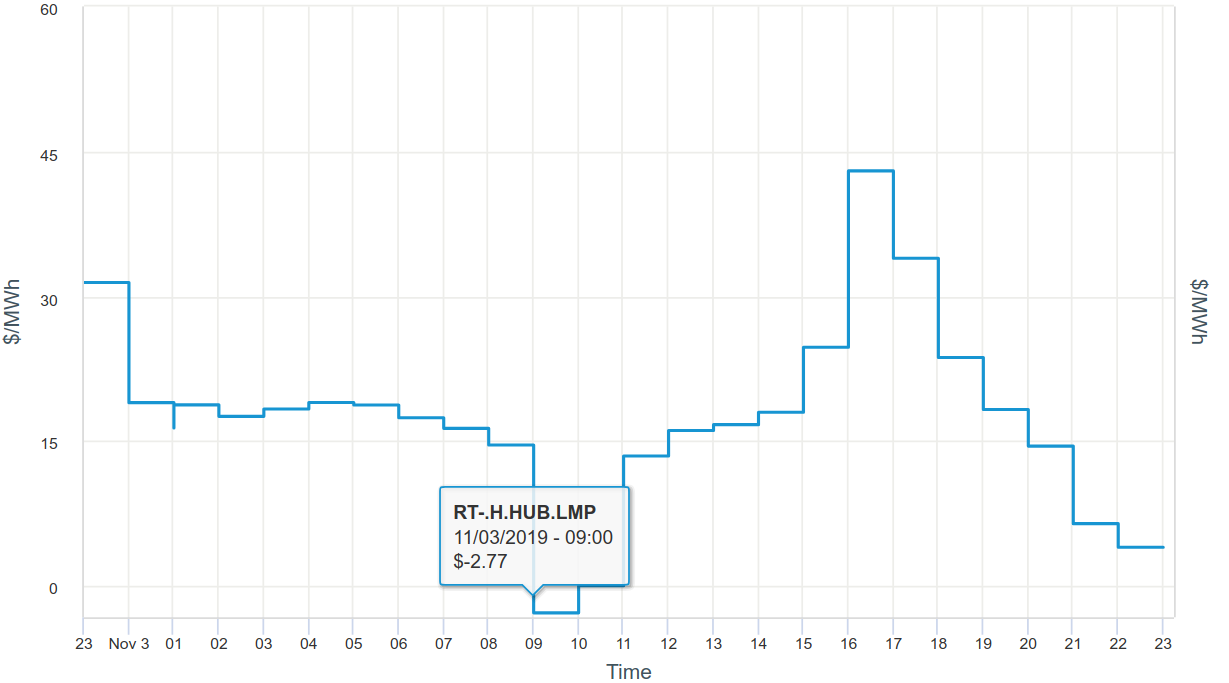
\includegraphics[width=0.65\textwidth]{./images/ne_one_day_price.png}
		\vspace{-2mm}
		\caption{ISO New England hourly electricity price; Nov 3, 2019 
			from 00:00AM to 11:00PM (Source: https://www.iso-ne.com/).}
	\end{figure}  
	\vspace{-4mm}
	
	\visible<2->{\begin{block}{Physical constraints limiting power 
	variations	in 
				Light-Water	Reactors \cite{lokhov_technical_2011}:}
			\begin{itemize}
				\item thermal strain and stress to fuel materials
				\item fuel burnup (insufficient excess reactivity at the 
				EOC)}
			\item<3-> \textbf{$^{135}Xe$ poisoning (iodine pit)}
		\end{itemize}
	\end{block}
\end{textblock*}
\end{frame}


\begin{frame}
\frametitle{What is $^{135}$Xe poisoning? \cite{nuclear_power_production_2020}}
\animategraphics[loop,controls,width=1.07\linewidth]{0.5}{./images/anime/xe_pois-}{0}{11}
\end{frame}


\begin{frame}
\frametitle{Postulated worst-case load-following scenario}
\vspace{-6mm}
\begin{columns}
	\column[t]{5.5cm}
	\begin{figure}[t]
		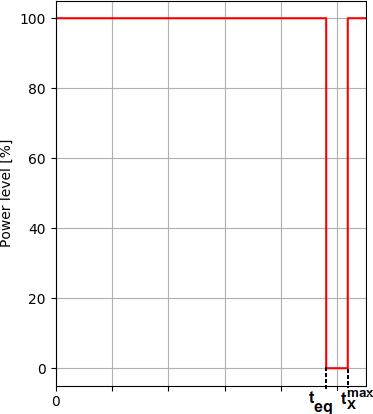
\includegraphics[width=\linewidth]{./images/power_load_curve.png}
		\vspace{-6mm}
		\caption{Postulated load-following power transient.}
	\end{figure}
	
	\column[t]{6.3cm}
	\begin{block}{Postulated load-following transient}
		\begin{enumerate}             
			\item $P(t<t_{eq})=100$\% to reach $^{135}$Xe/$^{135}$I equilibrium
			\item instantaneous power drop from 100 to 0\%
			\item $P(t_{eq}<t<t^{max}_{X})=0$\% to reach the 
			$^{135}$Xe peak
			\item restart instantly from 0 to 100\%, and then operation on 
			100\% for a few hours
		\end{enumerate}
			\vspace{-3mm}
	\end{block}
		{\footnotesize
		\begin{align}\label{eq:time-xe-max}
		t^{max}_{X} &= t_{eq} + \frac{1}{\lambda_X-\lambda_I}
		log\left(\frac{\lambda_X(\lambda_I[X_0+I_0]-\lambda_XX_0)}{\lambda_I^2 
		I_0}\right) \nonumber
		\end{align}}
				\vspace{-3mm}
	\begin{block}{Simplifying assumptions}
		\begin{itemize}
			\item All control rods are fully withdrawn
			\item Fission power adjusted by changing normalization in Serpent 
			2 ($\overline{\phi}=0$)
			\item 15-min depletion step
		\end{itemize}
		
	\end{block}
\end{columns}
\end{frame}

\begin{frame}
\frametitle{TAP load-following simulation without gas removal}
\begin{textblock*}{12.5cm}(0.1cm,2.1cm) % {block width} (coords)
\begin{columns}
	\column[t]{6.3cm}
	\begin{figure}[t]
		\begin{overprint}
	\onslide<2>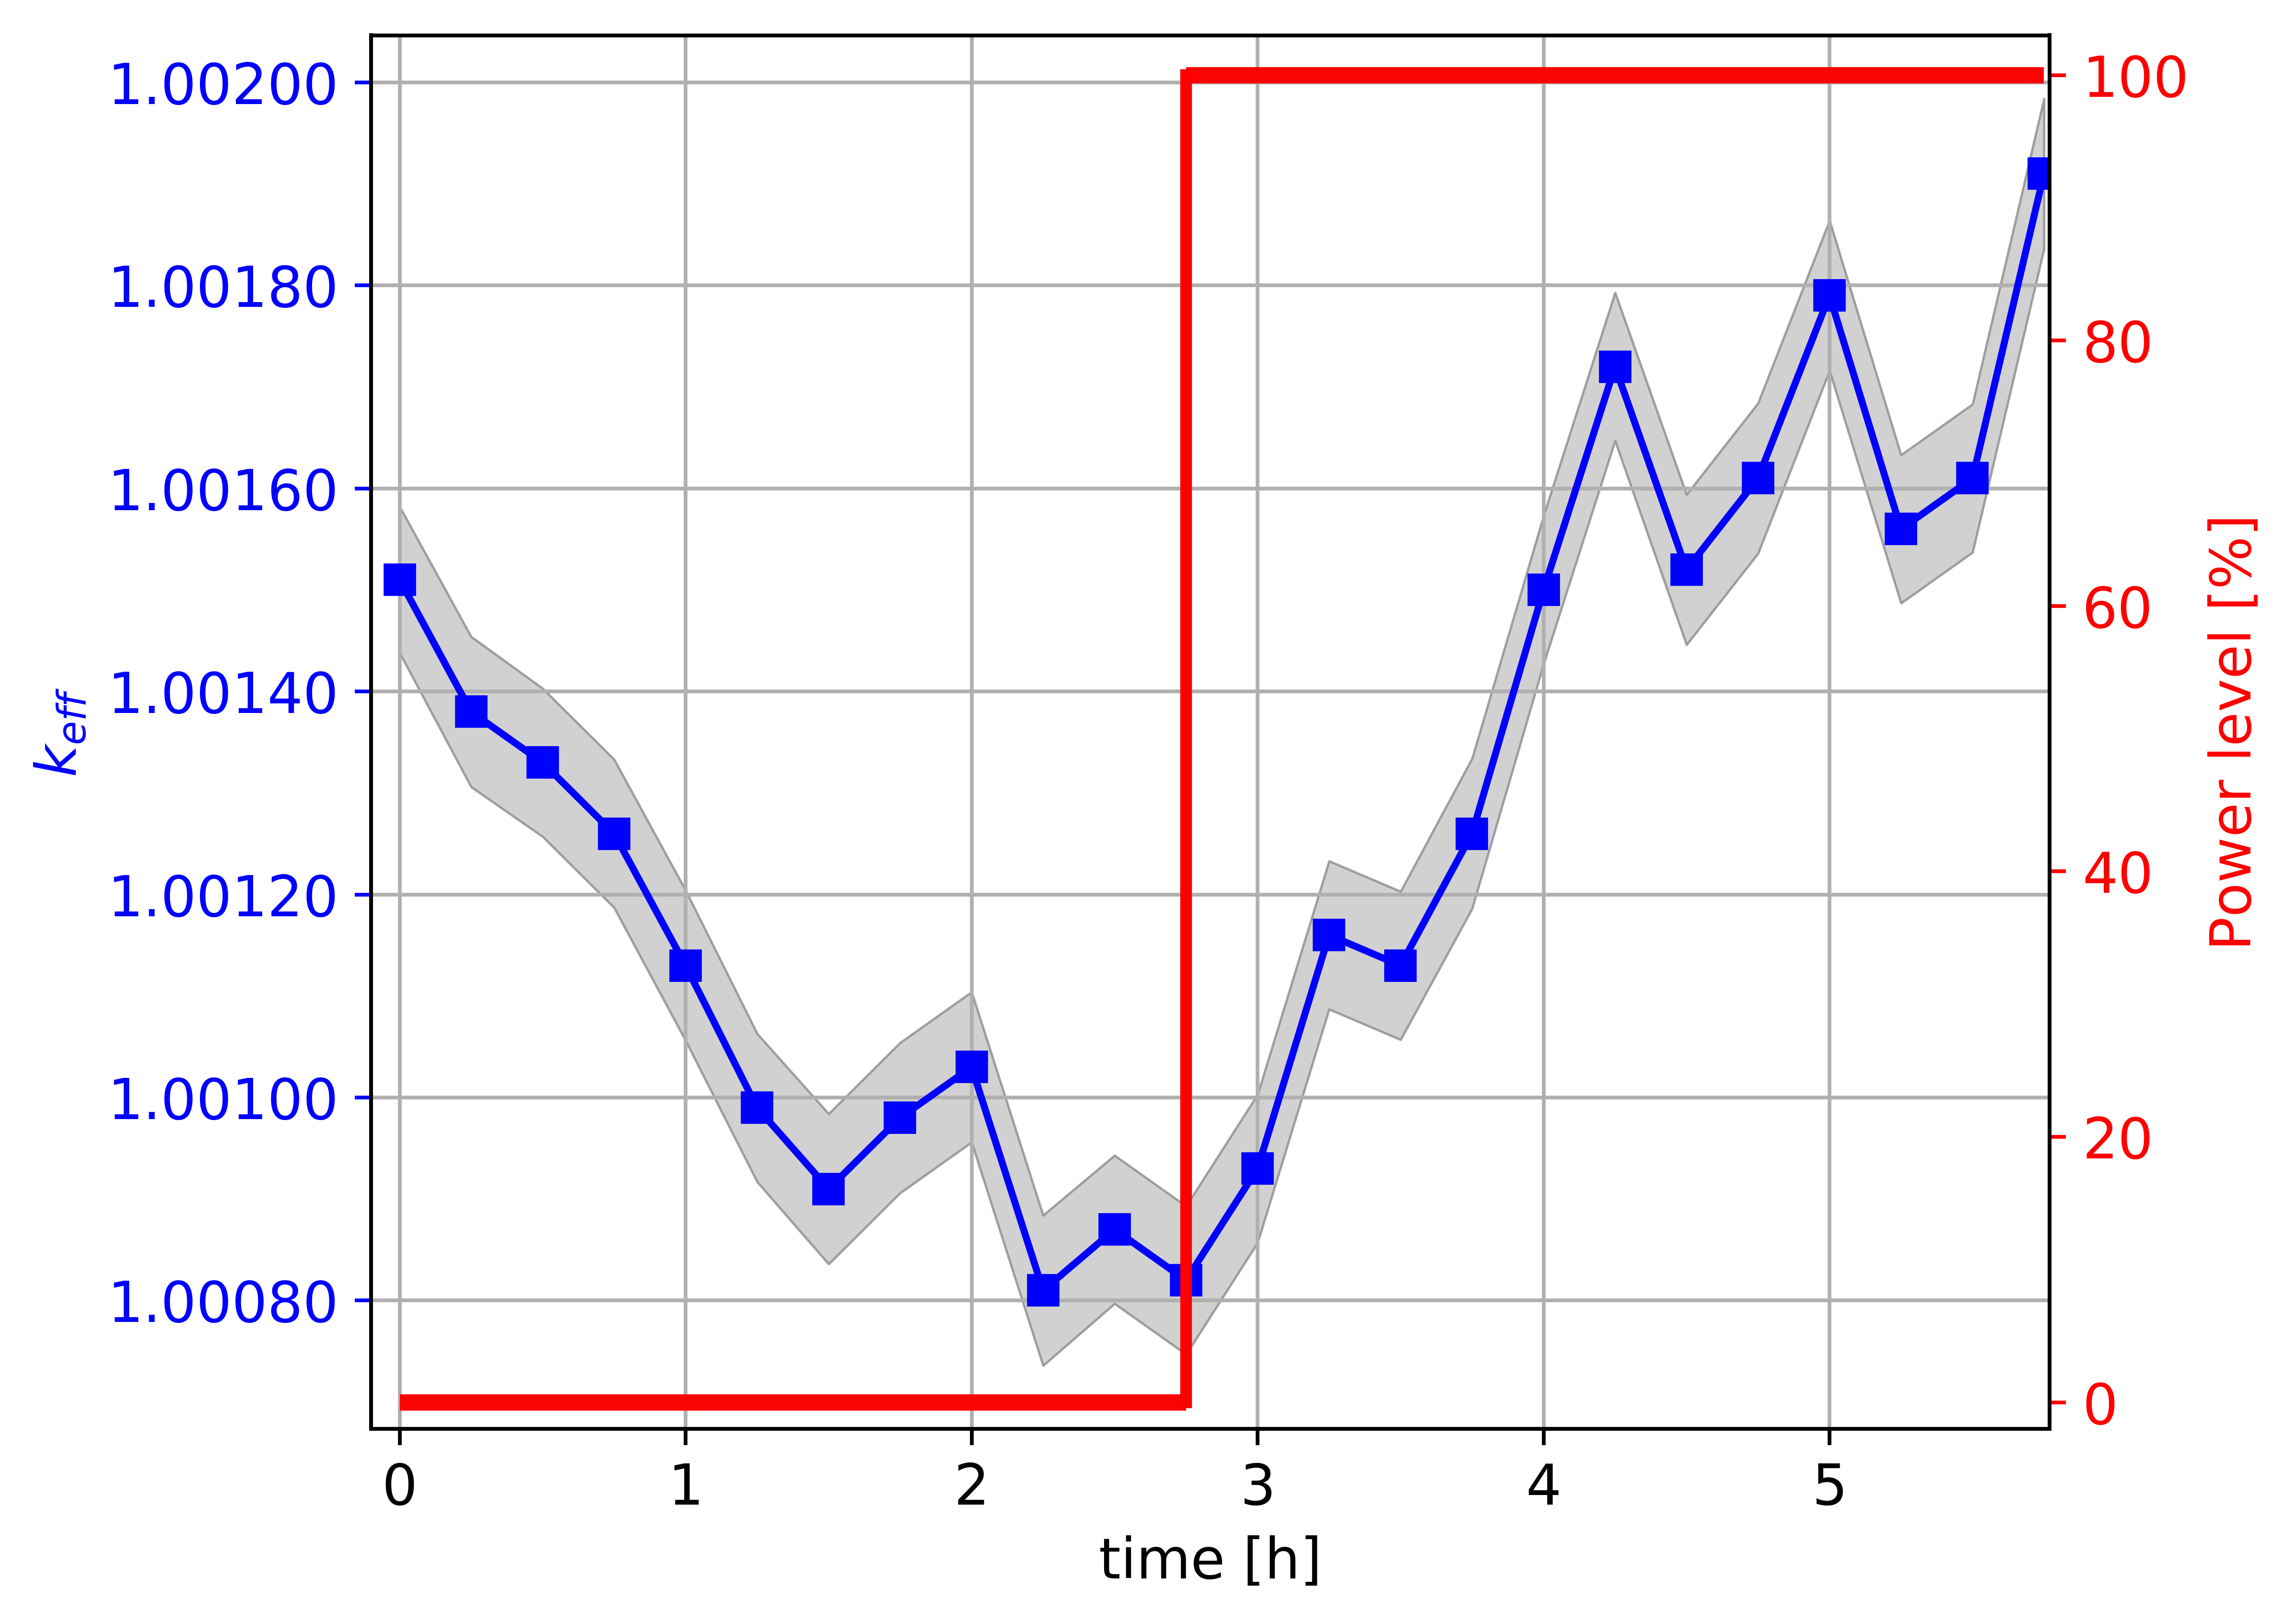
\includegraphics[width=1.11\linewidth]{../dissertation/figures/ch5/keff_kl_1_eol_eoc_15min.png}
		\vspace{-6mm}
	\caption{$k_{eff}$ dynamics during 2.75-hour shutdown (\textbf{10 days 
		before EOL}, \textbf{no gas removal}). $\sigma\pm7$ $pcm$ is shaded.}
	\onslide<3-4>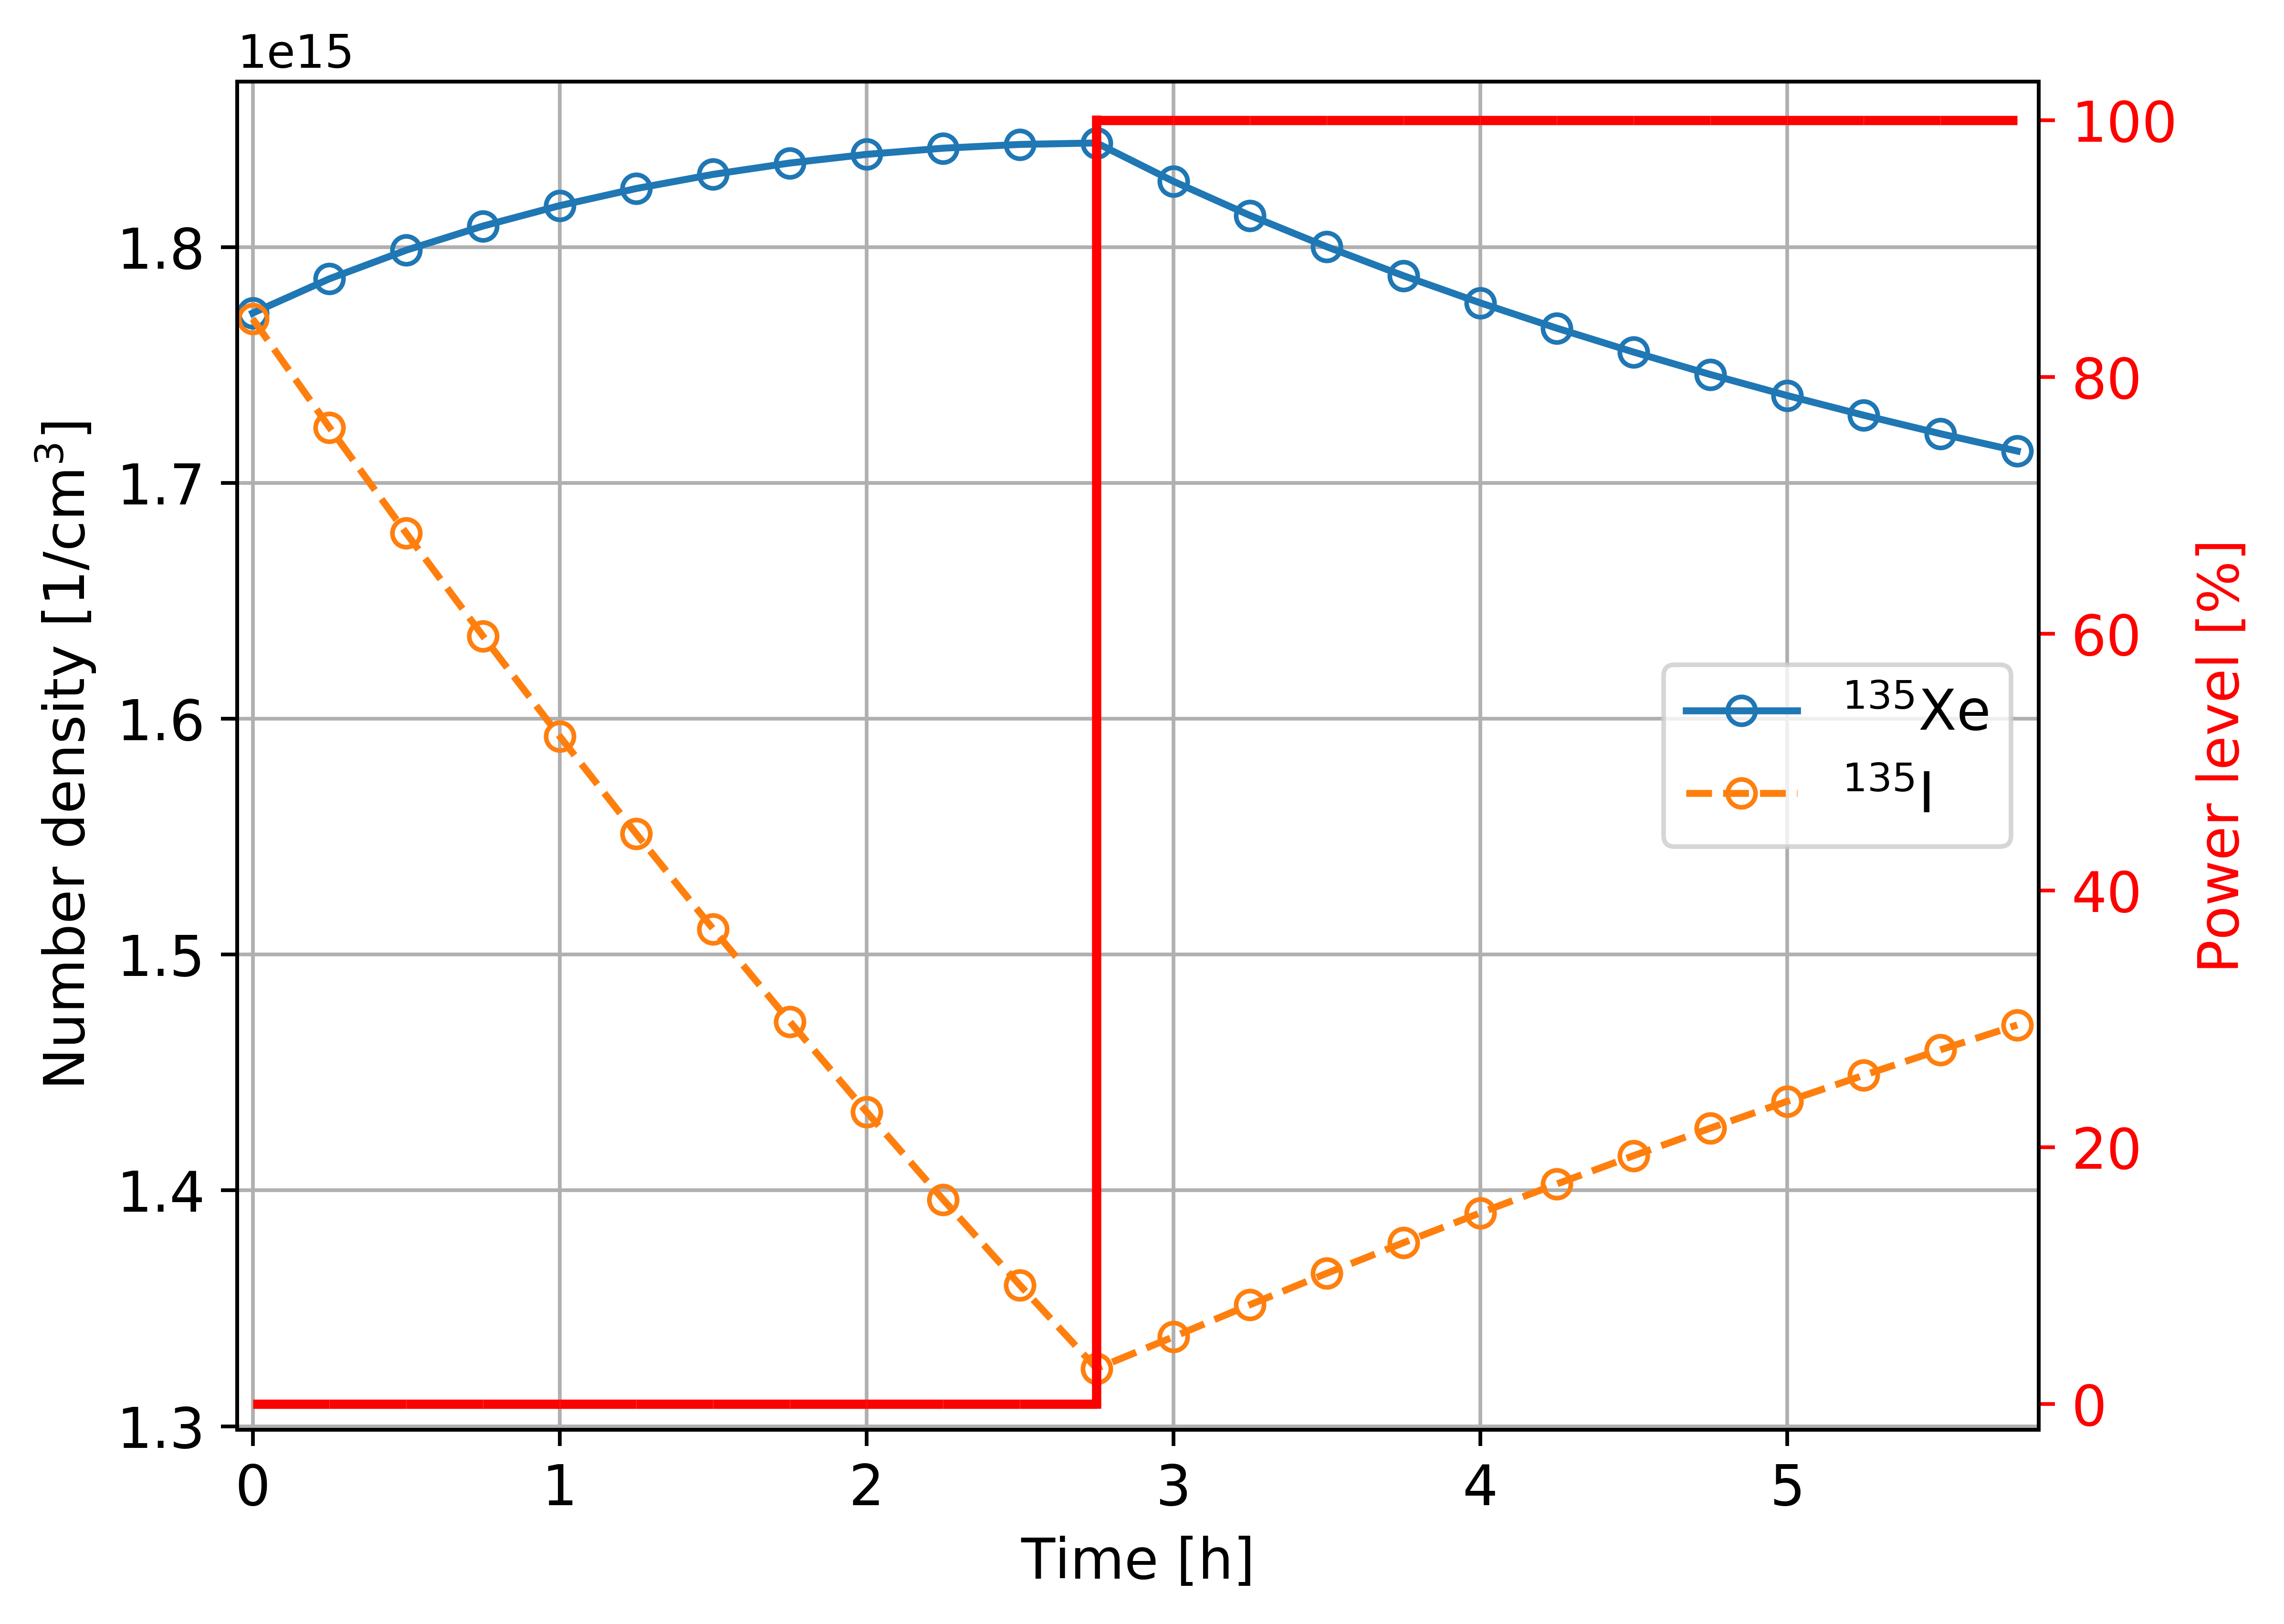
\includegraphics[width=1.11\linewidth]{../dissertation/figures/ch5/xe_i_kl_1_eol_eoc_15min.png}
		\vspace{-6mm}
	\caption{Number density of $^{135}$Xe and $^{135}$I during anticipated 
	transient (\textbf{10 days before EOL}, \textbf{no gas removal}).}
		\end{overprint}
	\end{figure}
	
	\column[t]{5.5cm}
	\begin{textblock*}{6cm}(6.65cm,2.1cm) % {block width} (coords)
		\fontsize{7}{9}\selectfont
		\begin{itemize}
		\item<1-> Negligible xenon poisoning at BOL
	\setbeamerfont*{itemize/enumerate body}{size=\footnotesize}
	\setbeamerfont*{itemize/enumerate subbody}{parent=itemize/enumerate 
	body}
	\setbeamerfont*{itemize/enumerate subsubbody}{parent=itemize/enumerate 
	body}			
			\begin{itemize}
				\item $\rho_X\approx-10\pm7$ $pcm$
				\item $^{135}$Xe concentration change $+0.33$\%
				\item $N_{^{135}I}/N_{^{135}Xe}<0.8$ due to hard spectrum
			\end{itemize} 
			\item<2-> Weak xenon poisoning at EOL (10d before shutdown, all 
			moderator rods are inserted)
	\setbeamerfont*{itemize/enumerate body}{size=\footnotesize}
	\setbeamerfont*{itemize/enumerate subbody}{parent=itemize/enumerate 
		body}
	\setbeamerfont*{itemize/enumerate subsubbody}{parent=itemize/enumerate 
		body}			
			\begin{itemize}
				\item $\rho_X\approx-70\pm7$ $pcm$
				\item<3-> $^{135}$Xe concentration change $+4$\%
				\item<3-> $N_{^{135}I}/N_{^{135}Xe}\approx1.0$
			\end{itemize}
		\end{itemize}
				\vspace{+5mm}
		\begin{block}<4->{\qquad Main takeaways}
			\begin{itemize}
				\item TAP \textbf{can load-follow} throughout whole
			lifetime \textbf{without significant $^{135}$Xe poisoning}
				\item Noble gas removal \textbf{unnecessary for load-following 
				in TAP}
				\item Noble gas removal \textbf{beneficial for long-term 
				performance}
				\item Main reason - \textbf{relatively fast neutron spectrum} 
				of TAP MSR
			\end{itemize}
		
	\end{block}
	\end{textblock*}
\end{columns}
\end{textblock*}
\end{frame}



\begin{frame}
\frametitle{Safety parameter evolution during load-following (EOL)}
\begin{textblock*}{12.5cm}(0.1cm,2.1cm) % {block width} (coords)
	\begin{columns}
		\column[t]{6.3cm}
		\begin{figure}[t]
			\begin{overprint}
	\onslide<1>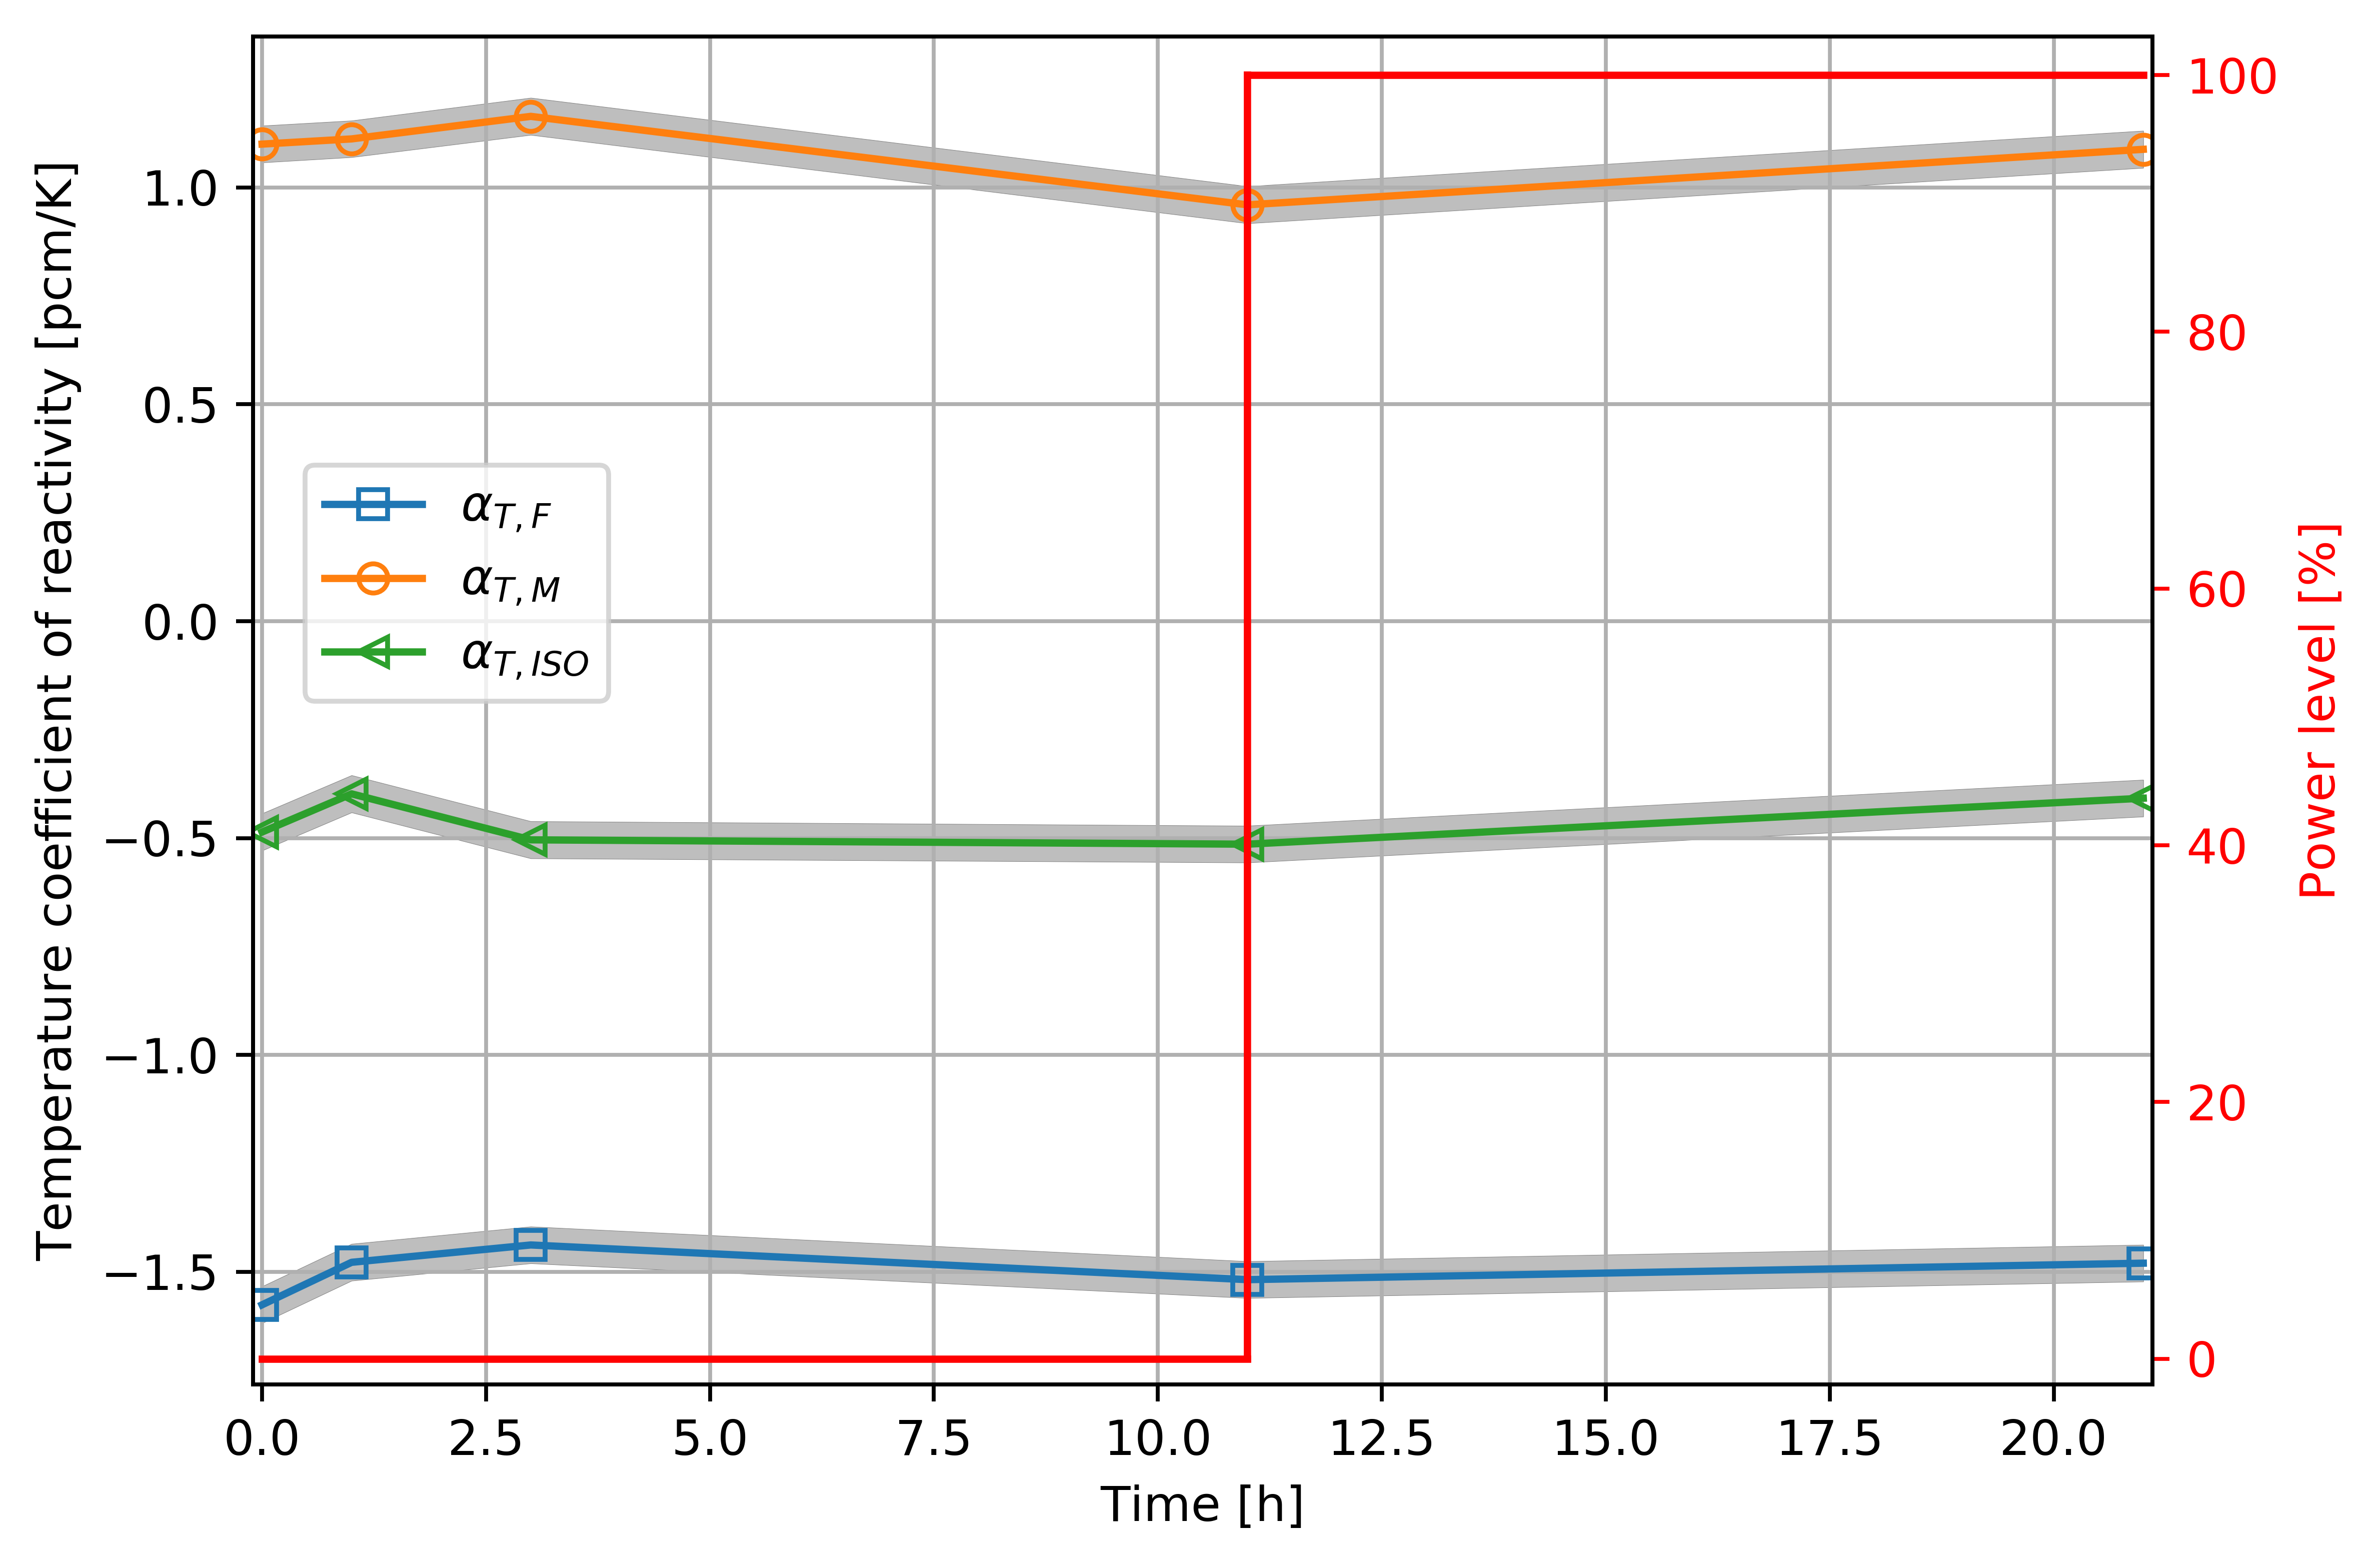
\includegraphics[width=1.15\linewidth]{../dissertation/figures/ch5/saf_par/tc_evo.png}
	\vspace{-6mm}
	\caption{Temperature feedback coefficients as a function of time during 
	the transient. 
	Uncertainty $\pm\sigma$ is shaded.}
	\onslide<2>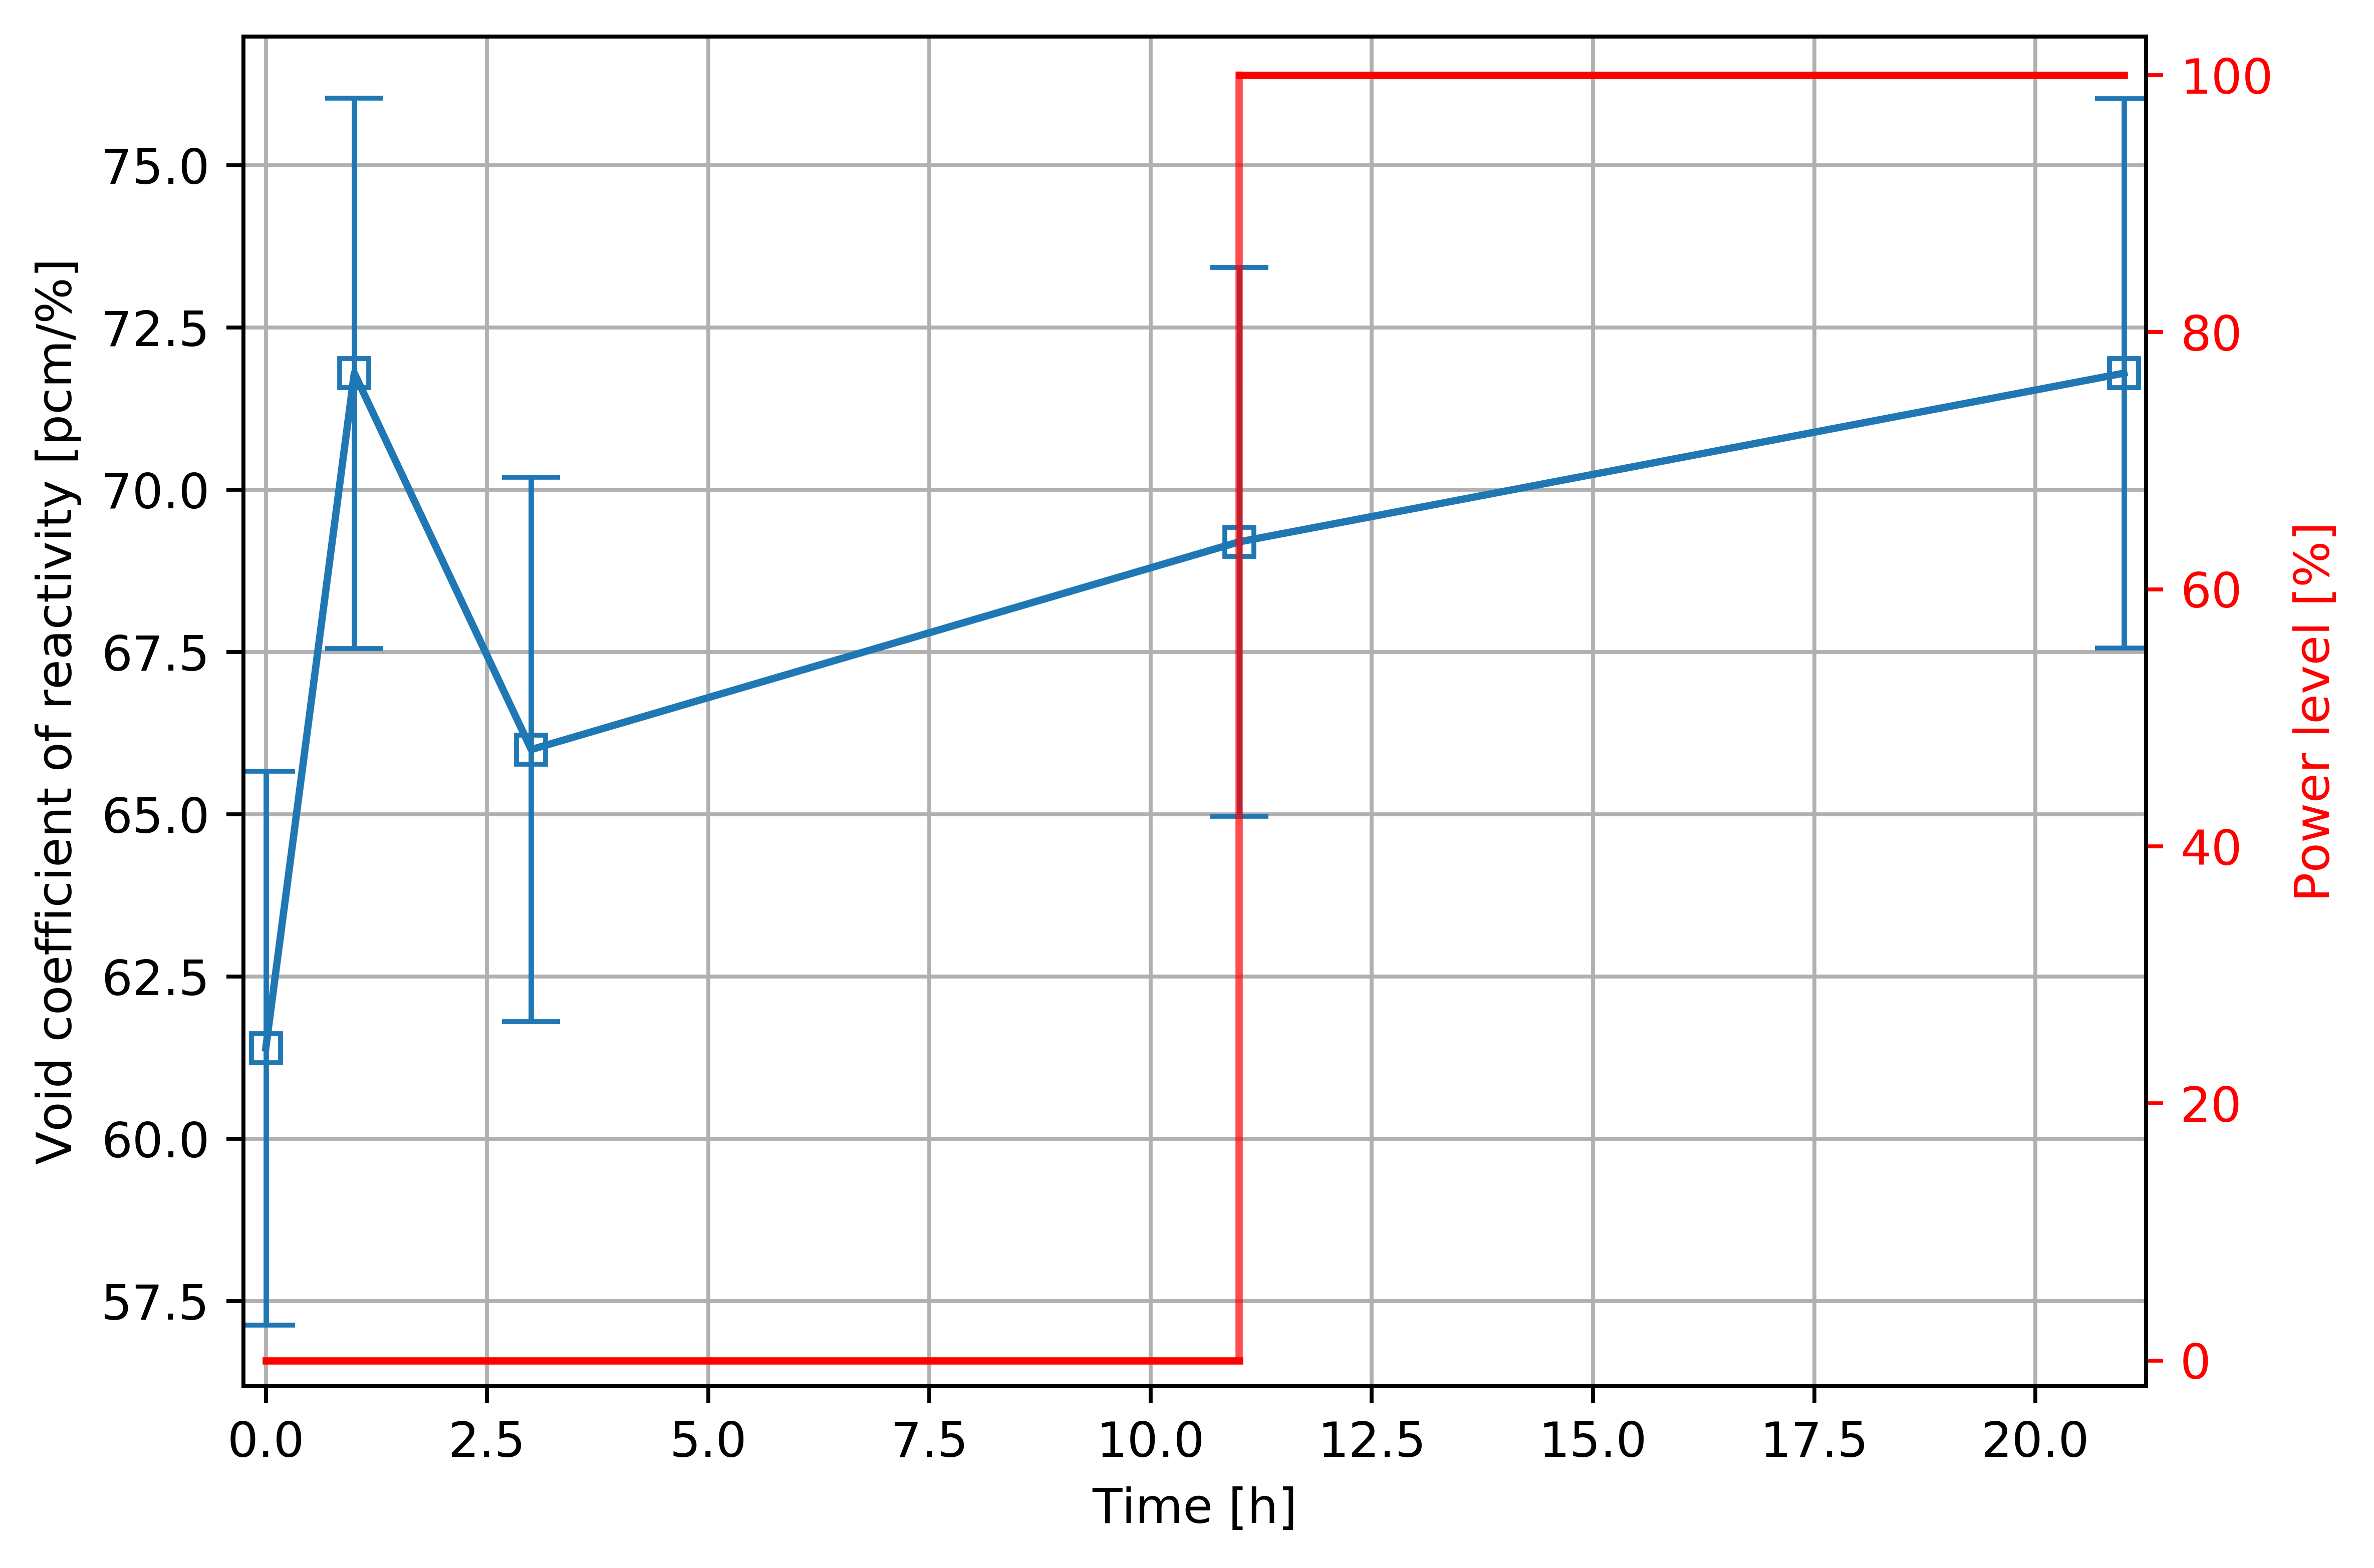
\includegraphics[width=1.15\linewidth]{../dissertation/figures/ch5/saf_par/void_evo.png}
	\vspace{-6mm}
	\caption{Void coefficient of reactivity ($\alpha_V$) as a function of time 
	during the transient.}
	\onslide<3->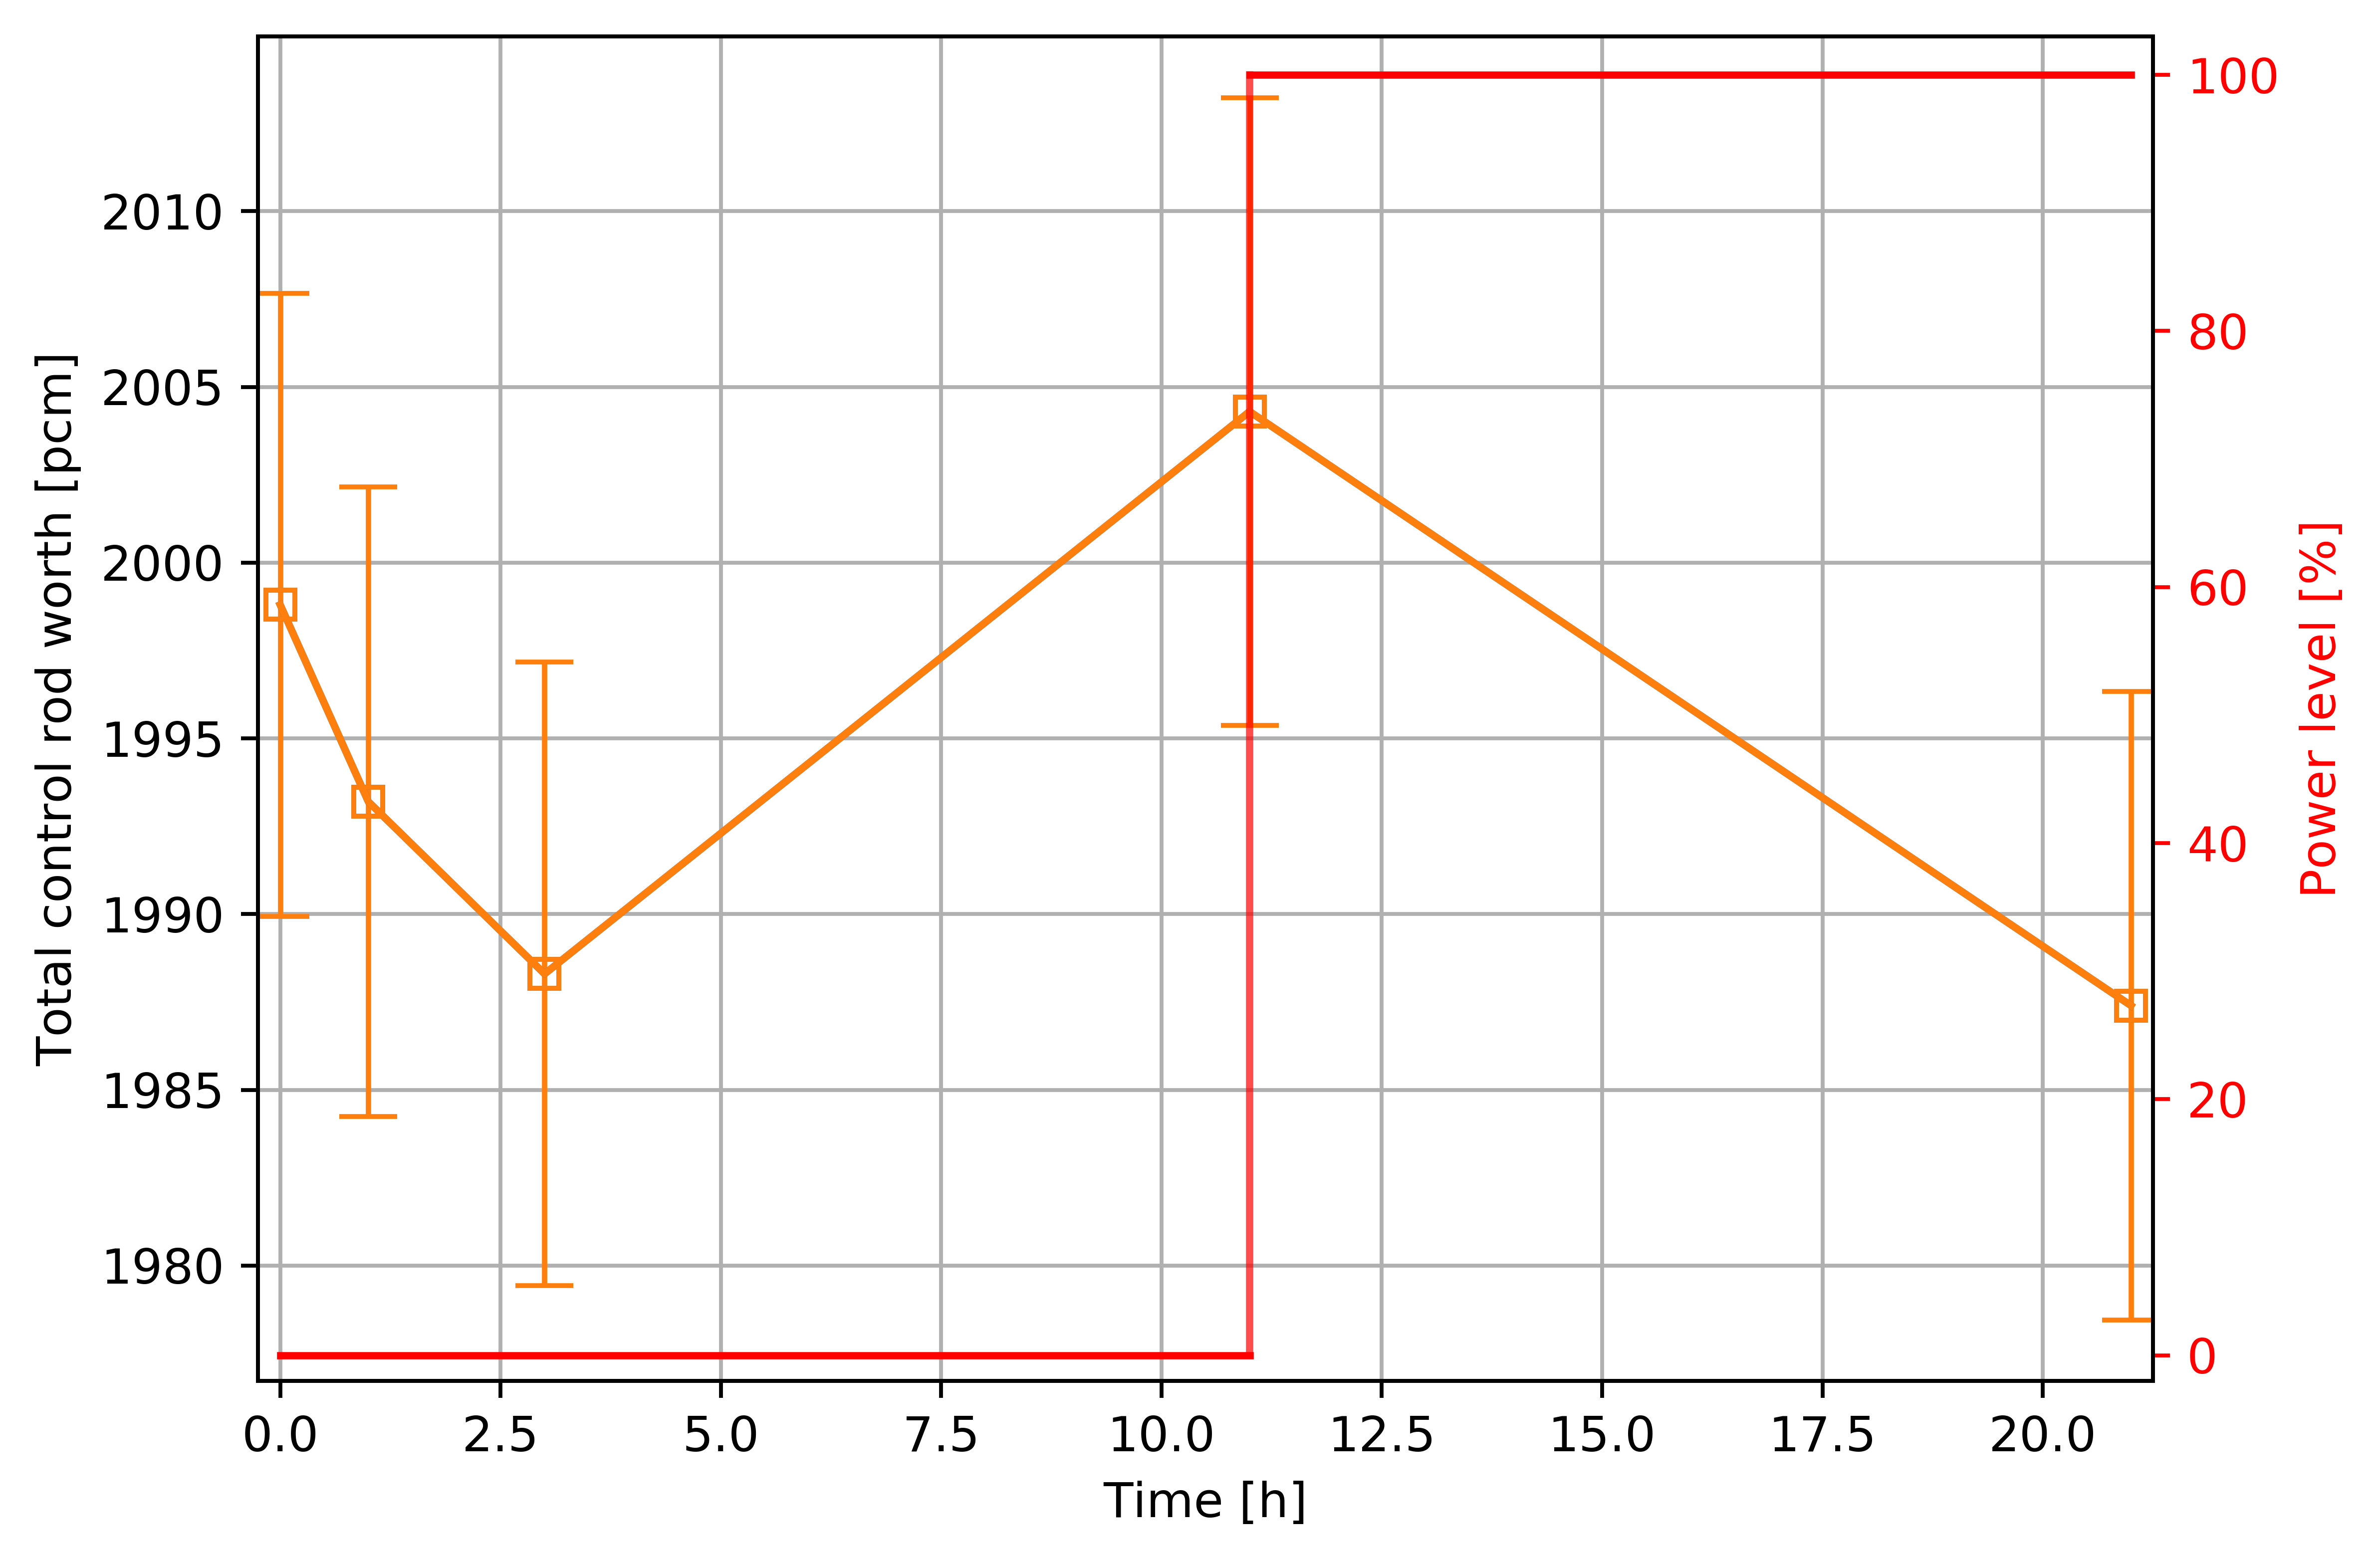
\includegraphics[width=1.15\linewidth]{../dissertation/figures/ch5/saf_par/crw_evo.png}
	\vspace{-6mm}
	\caption{Total control rod worth as a function of time during the 
	transient.}
			\end{overprint}
		\end{figure}
		
		\column[t]{5.5cm}
		\begin{textblock*}{5.9cm}(6.9cm,2.6cm) % {block width} (coords)
			\begin{itemize}
				\itemsep=0.8em
				\item<1-> Fuel temperature coefficient ($\alpha_{T,F}$) 
				worsened during first 3 hours when $^{135}$Xe concentration 
				peaked causing the spectrum hardening
				\item<2-> $\alpha_V$ fluctuates in stochastic uncertainty 
				range $\sigma_{\alpha_V}\pm4$ $pcm/$\%
				\item<3-> CRW worsened right after shutdown but then quickly 
				recovered due to quick $^{135}$Xe removal
				\item<4-> TAP reactor maintains safety margins during the 
				load-following transient
			\end{itemize}
				
		\end{textblock*}
	\end{columns}
\end{textblock*}
\end{frame}


\subsection{Short-term depletion: MSBR}

\begin{frame}
\frametitle{Xenon poisoning effect during MSBR load-following}
\vspace{-8mm}
\begin{columns}
	\column[t]{7cm}
	\visible<2->{
	\begin{figure}[t]
	\centering
$\begin{array}{r}
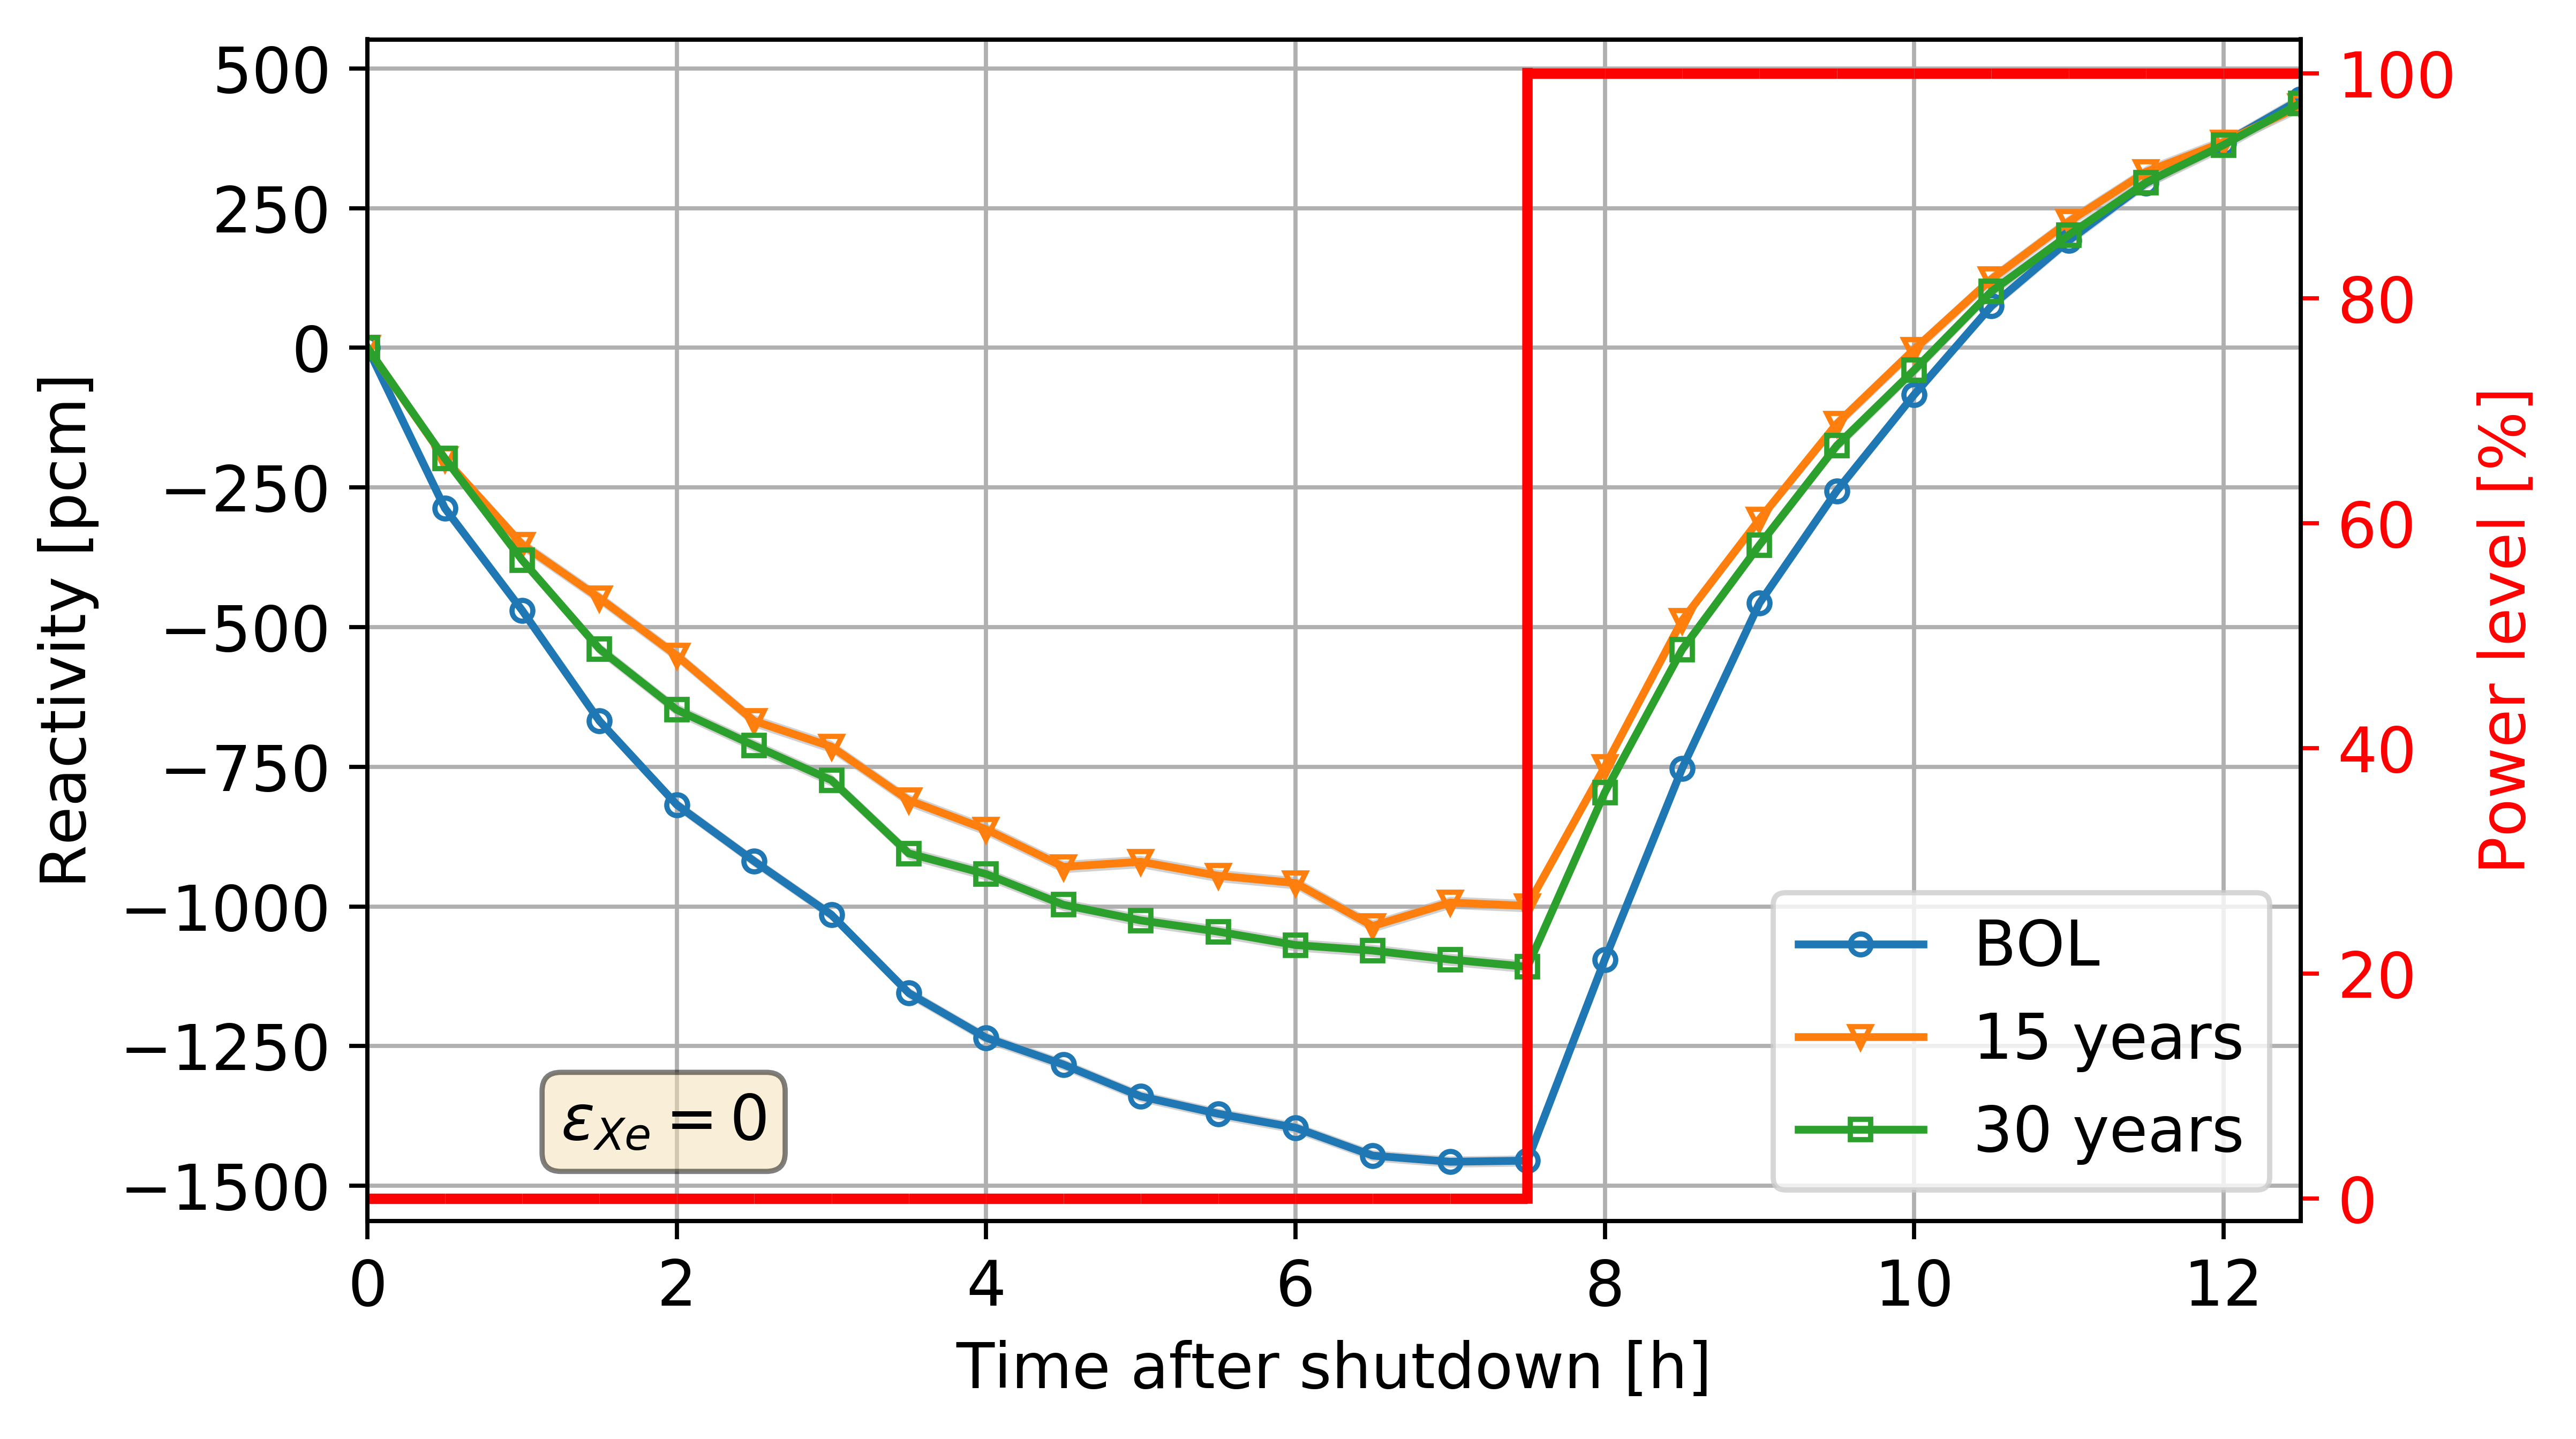
\includegraphics[width=0.717\textwidth]{../dissertation/figures/ch6/kl1_rho.png}\vspace{-5mm}\\
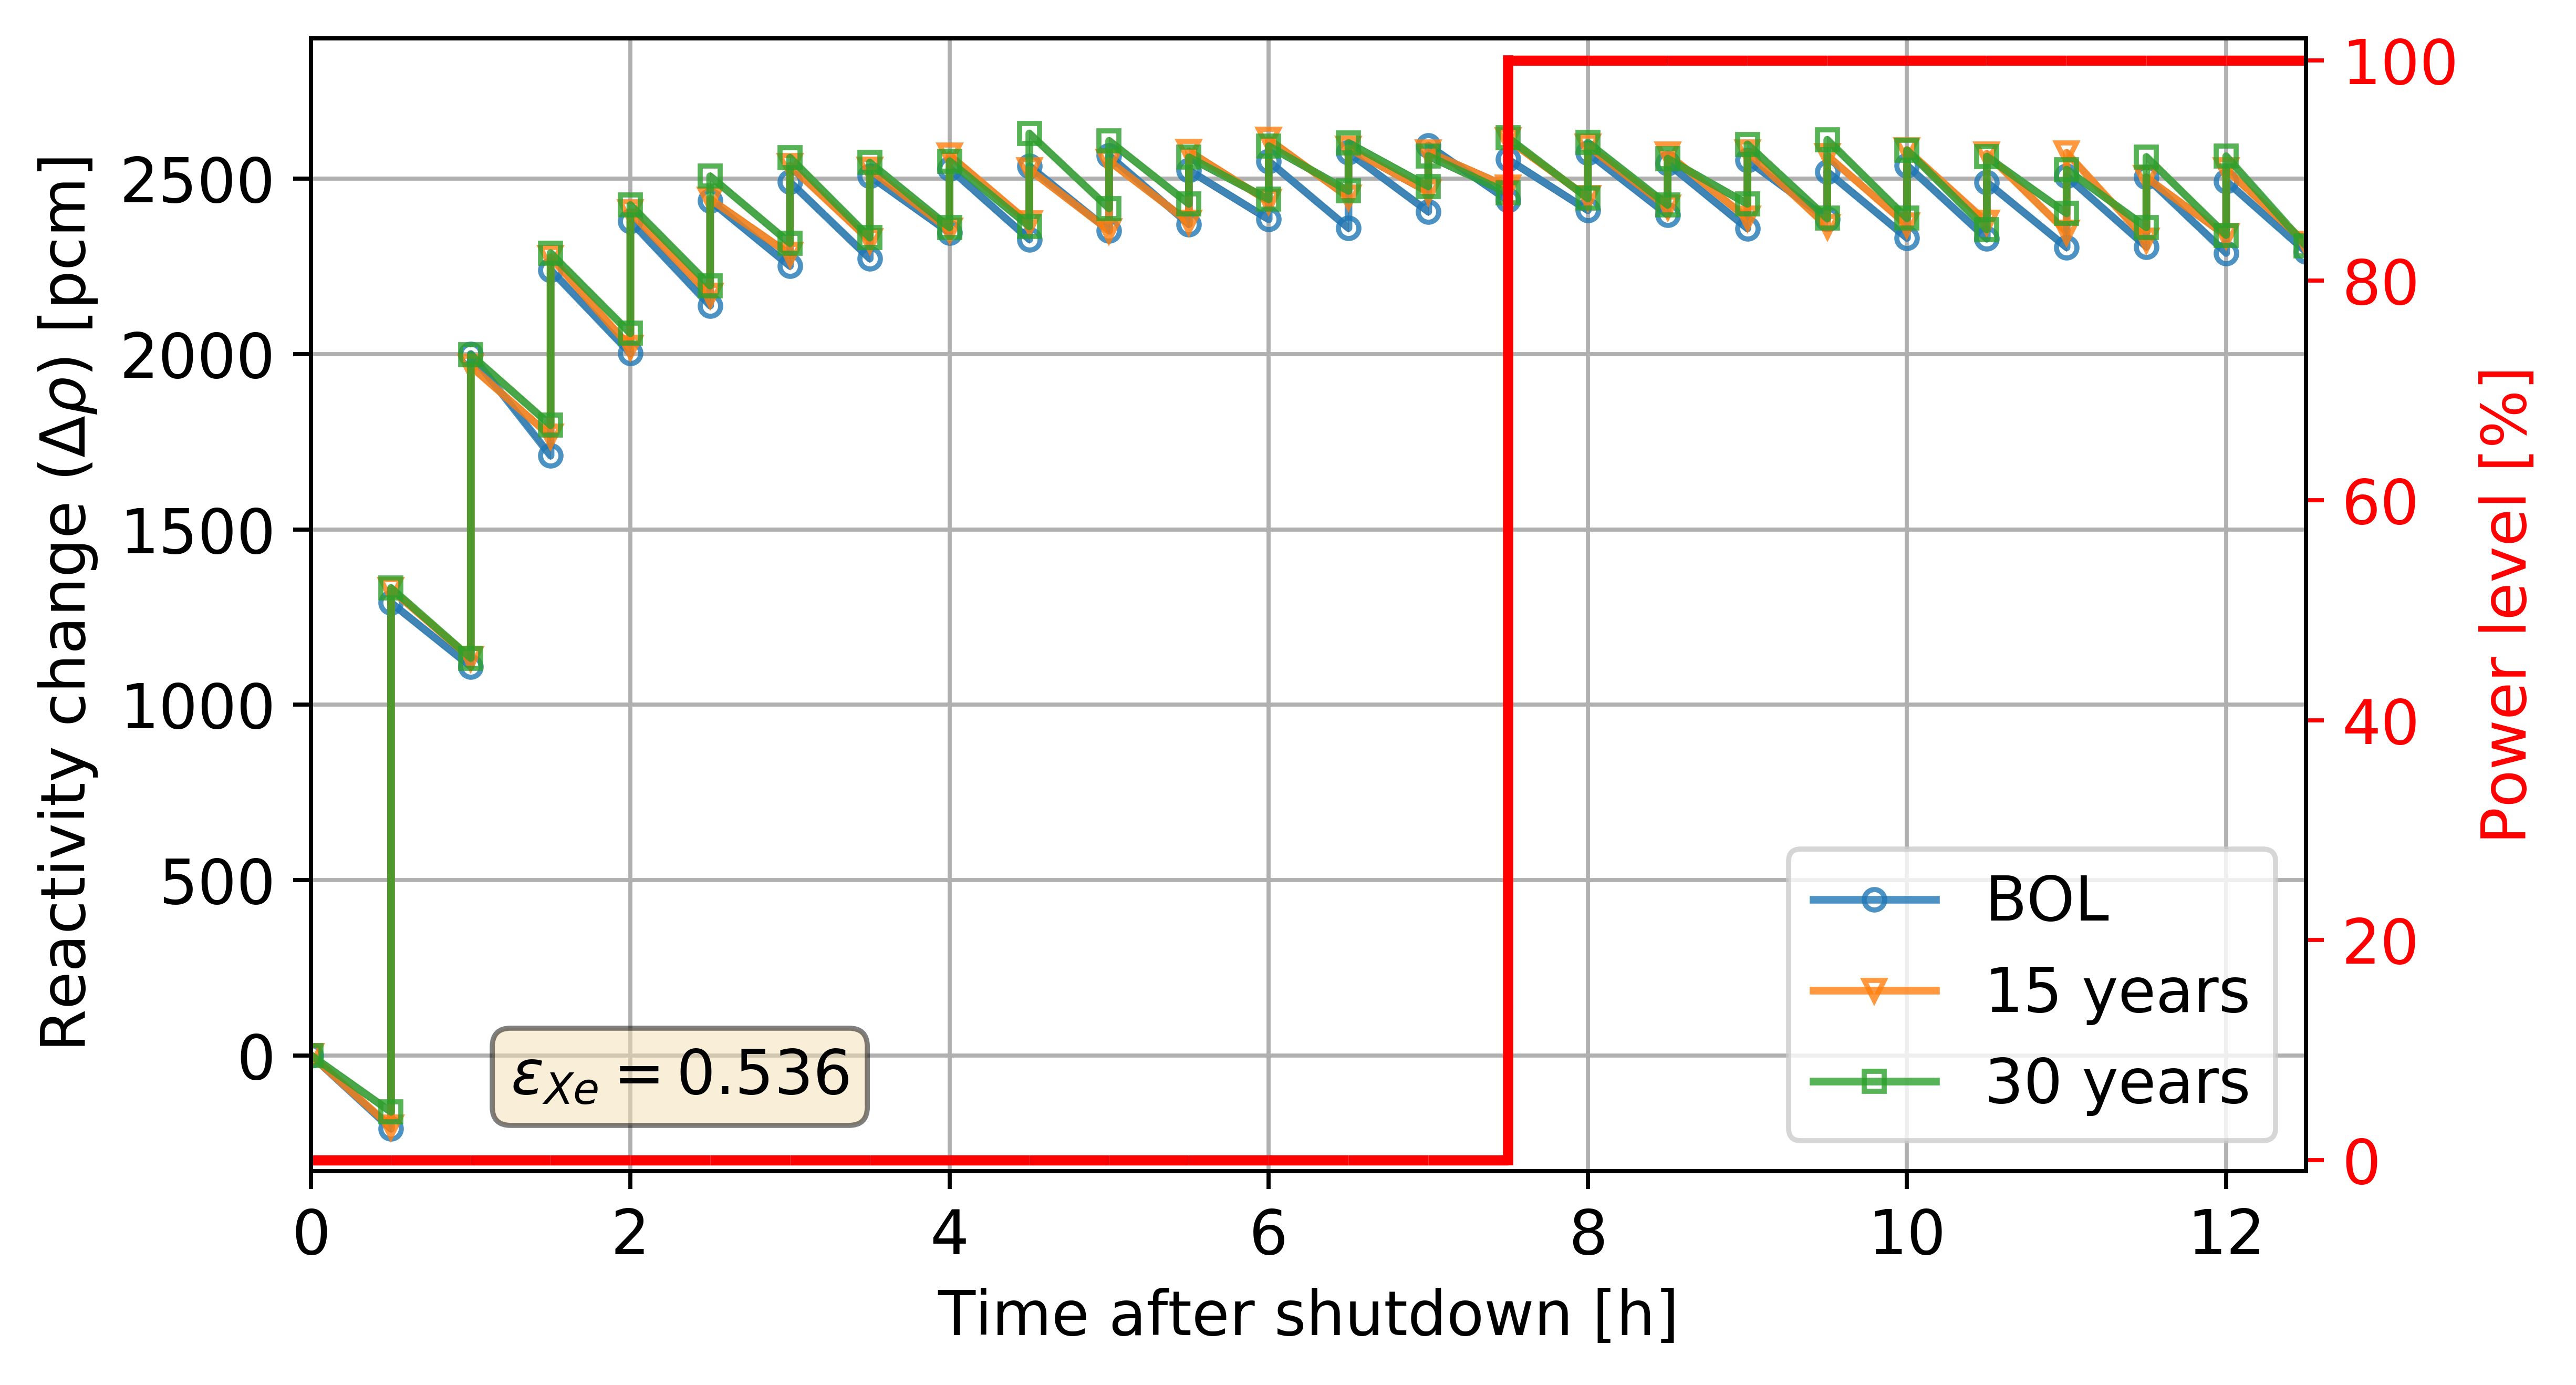
\includegraphics[width=0.70\textwidth]{../dissertation/figures/ch6/kl25_rho.png}\vspace{-5mm}\\
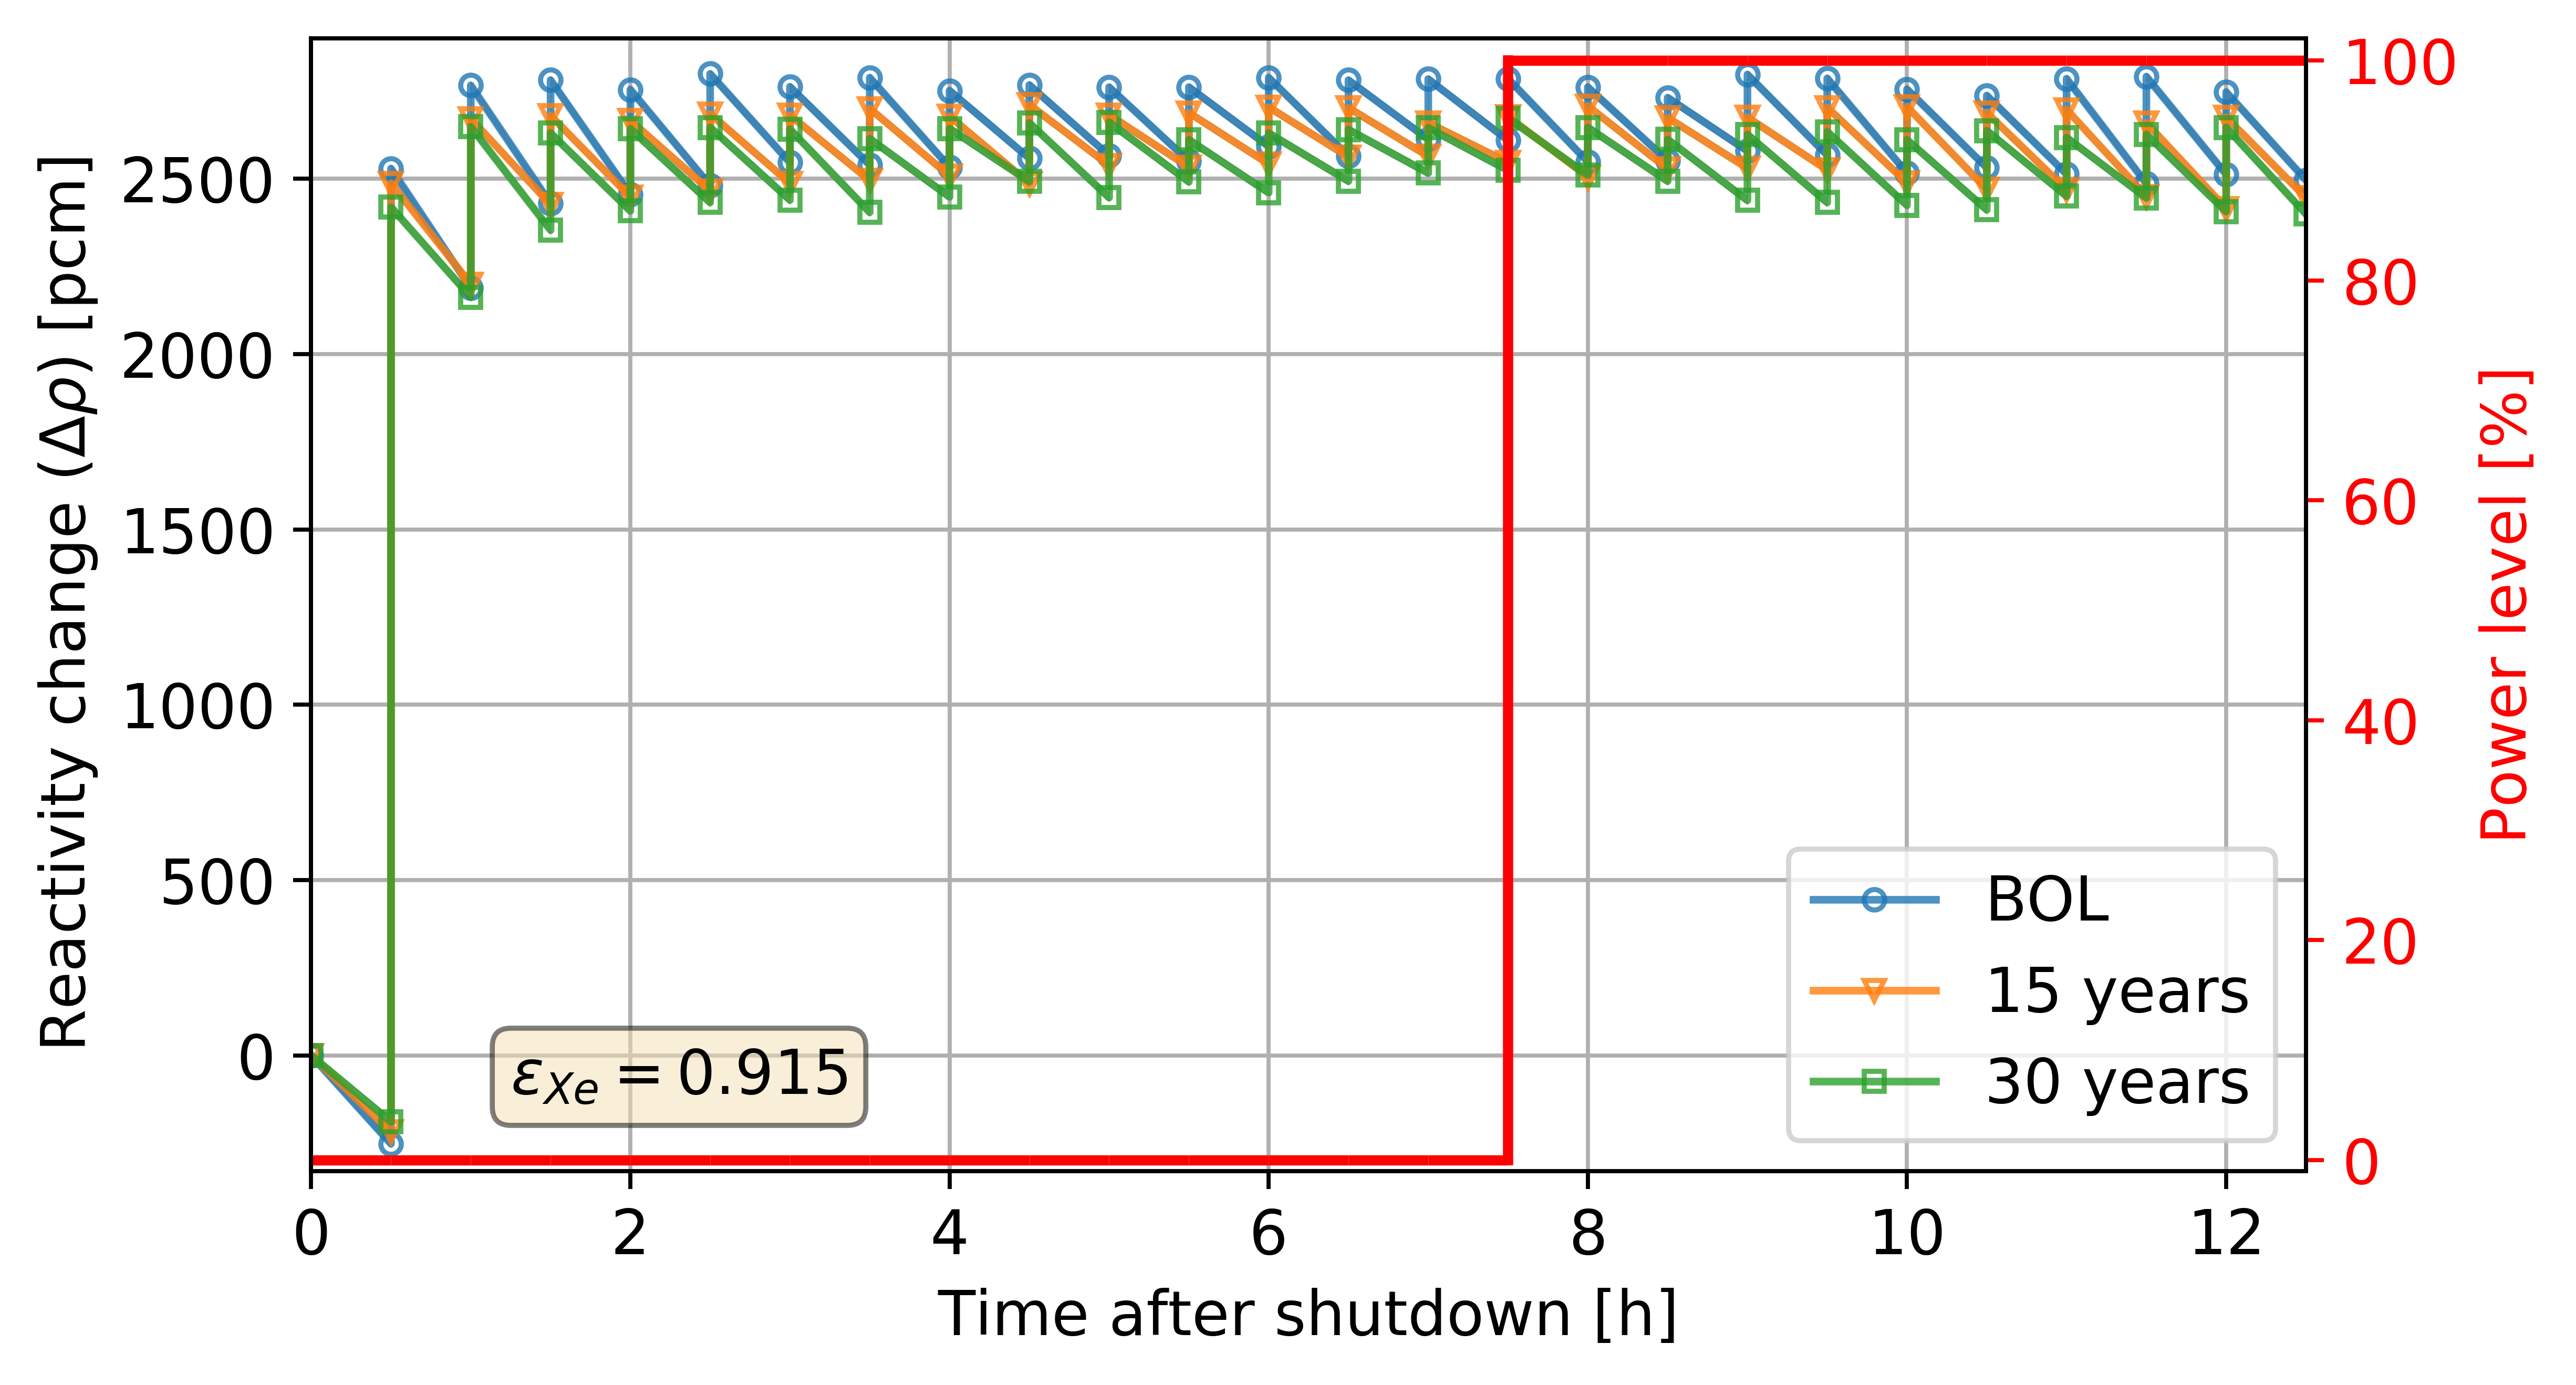
\includegraphics[width=0.70\textwidth]{../dissertation/figures/ch6/kl100_rho.png}
\end{array}$
\vspace{-4mm}
\caption{$\rho(t)$ during the transient ($\pm\sigma_{\rho}=10$$pcm$).}
	\end{figure}}
	
	\column[t]{5.5cm}
	\begin{textblock*}{6.1cm}(6.3cm,2cm) % {block width} (coords)
	\begin{block}<1->{Analysis assumptions}
				\fontsize{7}{9}\selectfont
		\begin{enumerate}             
			\item Load profile similar to TAP reactor
			\item $t^{max}_X\approx7.5h$
			\item 30-min depletion step
			\item Low, medium, and high gas removal efficiency
		\end{enumerate}
		\vspace{-1mm}
	\end{block}

	\begin{block}<2->{Key takeaways}
				\fontsize{7}{9}\selectfont
		\begin{itemize}
			\item MSBR \textbf{cannot load-follow without gas removal:} 
			$\Delta\rho=-1490pcm$
			\item Xenon poisoning is \textbf{milder toward EOL} due to 
			spectrum \textbf{hardening}
			\item Huge \textbf{positive reactivity insertion} for medium 
			and high removal efficiency
			\item Even removal of \textbf{53.6\%} of Xe significantly 
			reduced the effect of poisoning: \textbf{-161$\pm10pcm$}
			\item More effective removal (\textbf{91.5\%}) gave similar 
			improvement: \textbf{-189$\pm10pcm$}
		\end{itemize}
		
	\end{block}
\end{textblock*}
\end{columns}
\end{frame}

\begin{frame}
\frametitle{Safety parameter evolution during load-following}
\begin{textblock*}{12.5cm}(0.4cm,1.55cm) % {block width} (coords)
	\begin{columns}
		\column[t]{6.3cm}
		\begin{figure}[t]
			\begin{overprint}
				\onslide<1>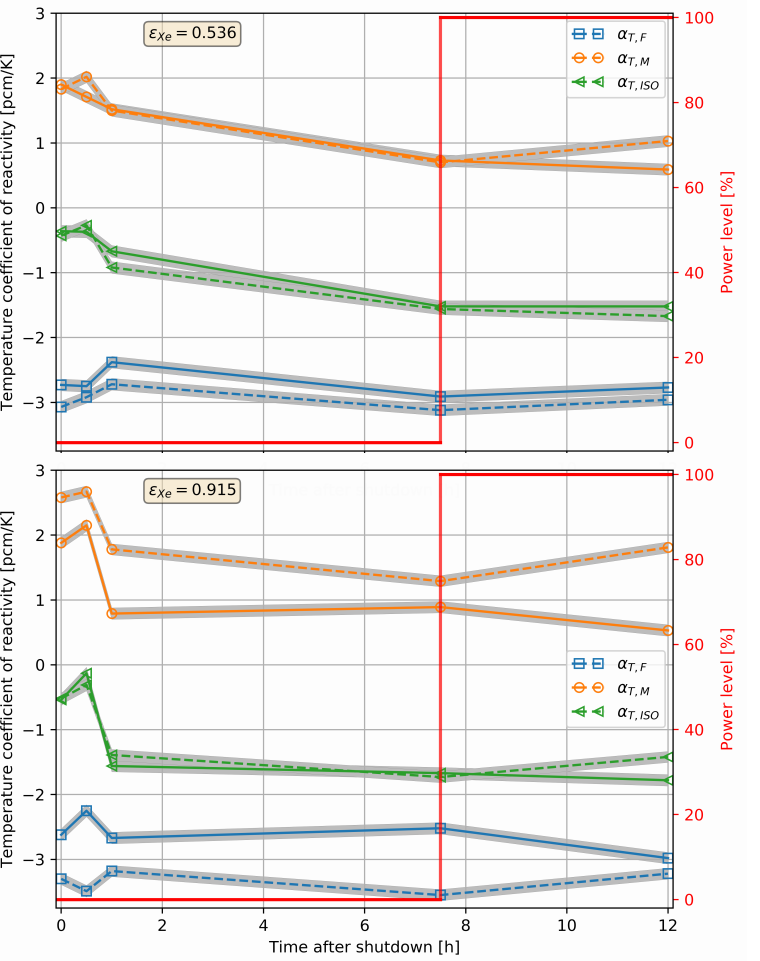
\includegraphics[width=0.87\linewidth]{./images/msbr_tc_evo.png}
				\vspace{-2mm}
				\caption{Temperature coefficients dynamics during the 
				transient.}
				\onslide<2>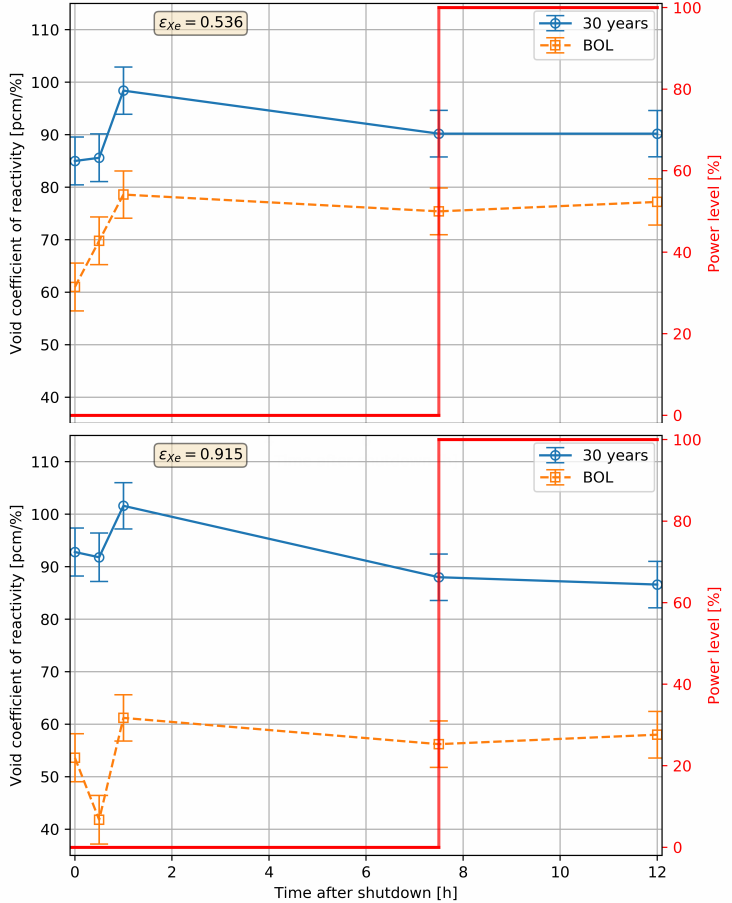
\includegraphics[width=0.87\linewidth]{./images/msbr_void_evo.png}
				\vspace{-1mm}
				\caption{Void coefficient of reactivity ($\alpha_V$) dynamics
					during the transient.}
				\onslide<3->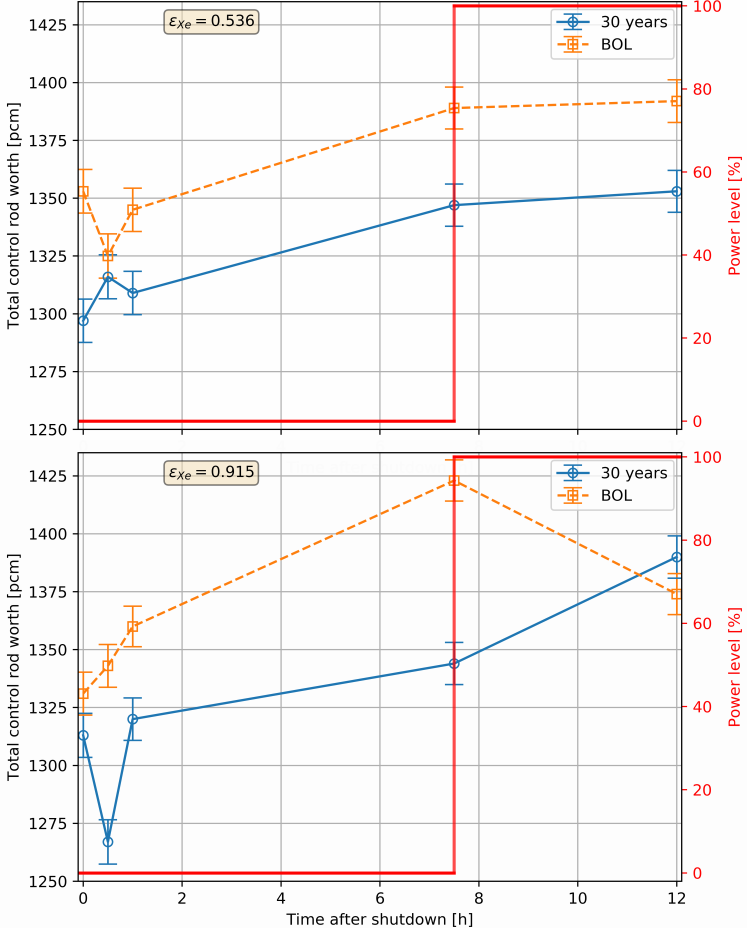
\includegraphics[width=0.87\linewidth]{./images/msbr_crw_evo.png}
				\vspace{-1mm}
				\caption{Total control rod worth dynamics during 
				the transient.}
			\end{overprint}
		\end{figure}
		
		\column[t]{6cm}
		\begin{textblock*}{6.7cm}(6cm,2.6cm) % {block width} (coords)
			\begin{itemize}
				\itemsep=0.8em
				\item<1-> $\alpha_{T,ISO}$ worsens slightly as $^{135}$Xe 
				concentration spikes and then improves quickly
				\item<2-> $\alpha_V$ demonstrates similar behavior
				\item<3-> CRW worsens after shutdown but then quickly 
				improves due to quick $^{135}$Xe removal
				\item<4-> Total control rod worth is insufficient to shut down 
				the reactor at any time during transient
			\end{itemize}
			
		\end{textblock*}
	\end{columns}
\end{textblock*}
\end{frame}


\begin{frame}
\frametitle{Neutron energy spectrum MSBR vs TAP}
\begin{textblock*}{12.6cm}(0.1cm,1.6cm) % {block width} (coords)
	\begin{figure}[htp!] % replace 't' with 'b' to 
		\centerline{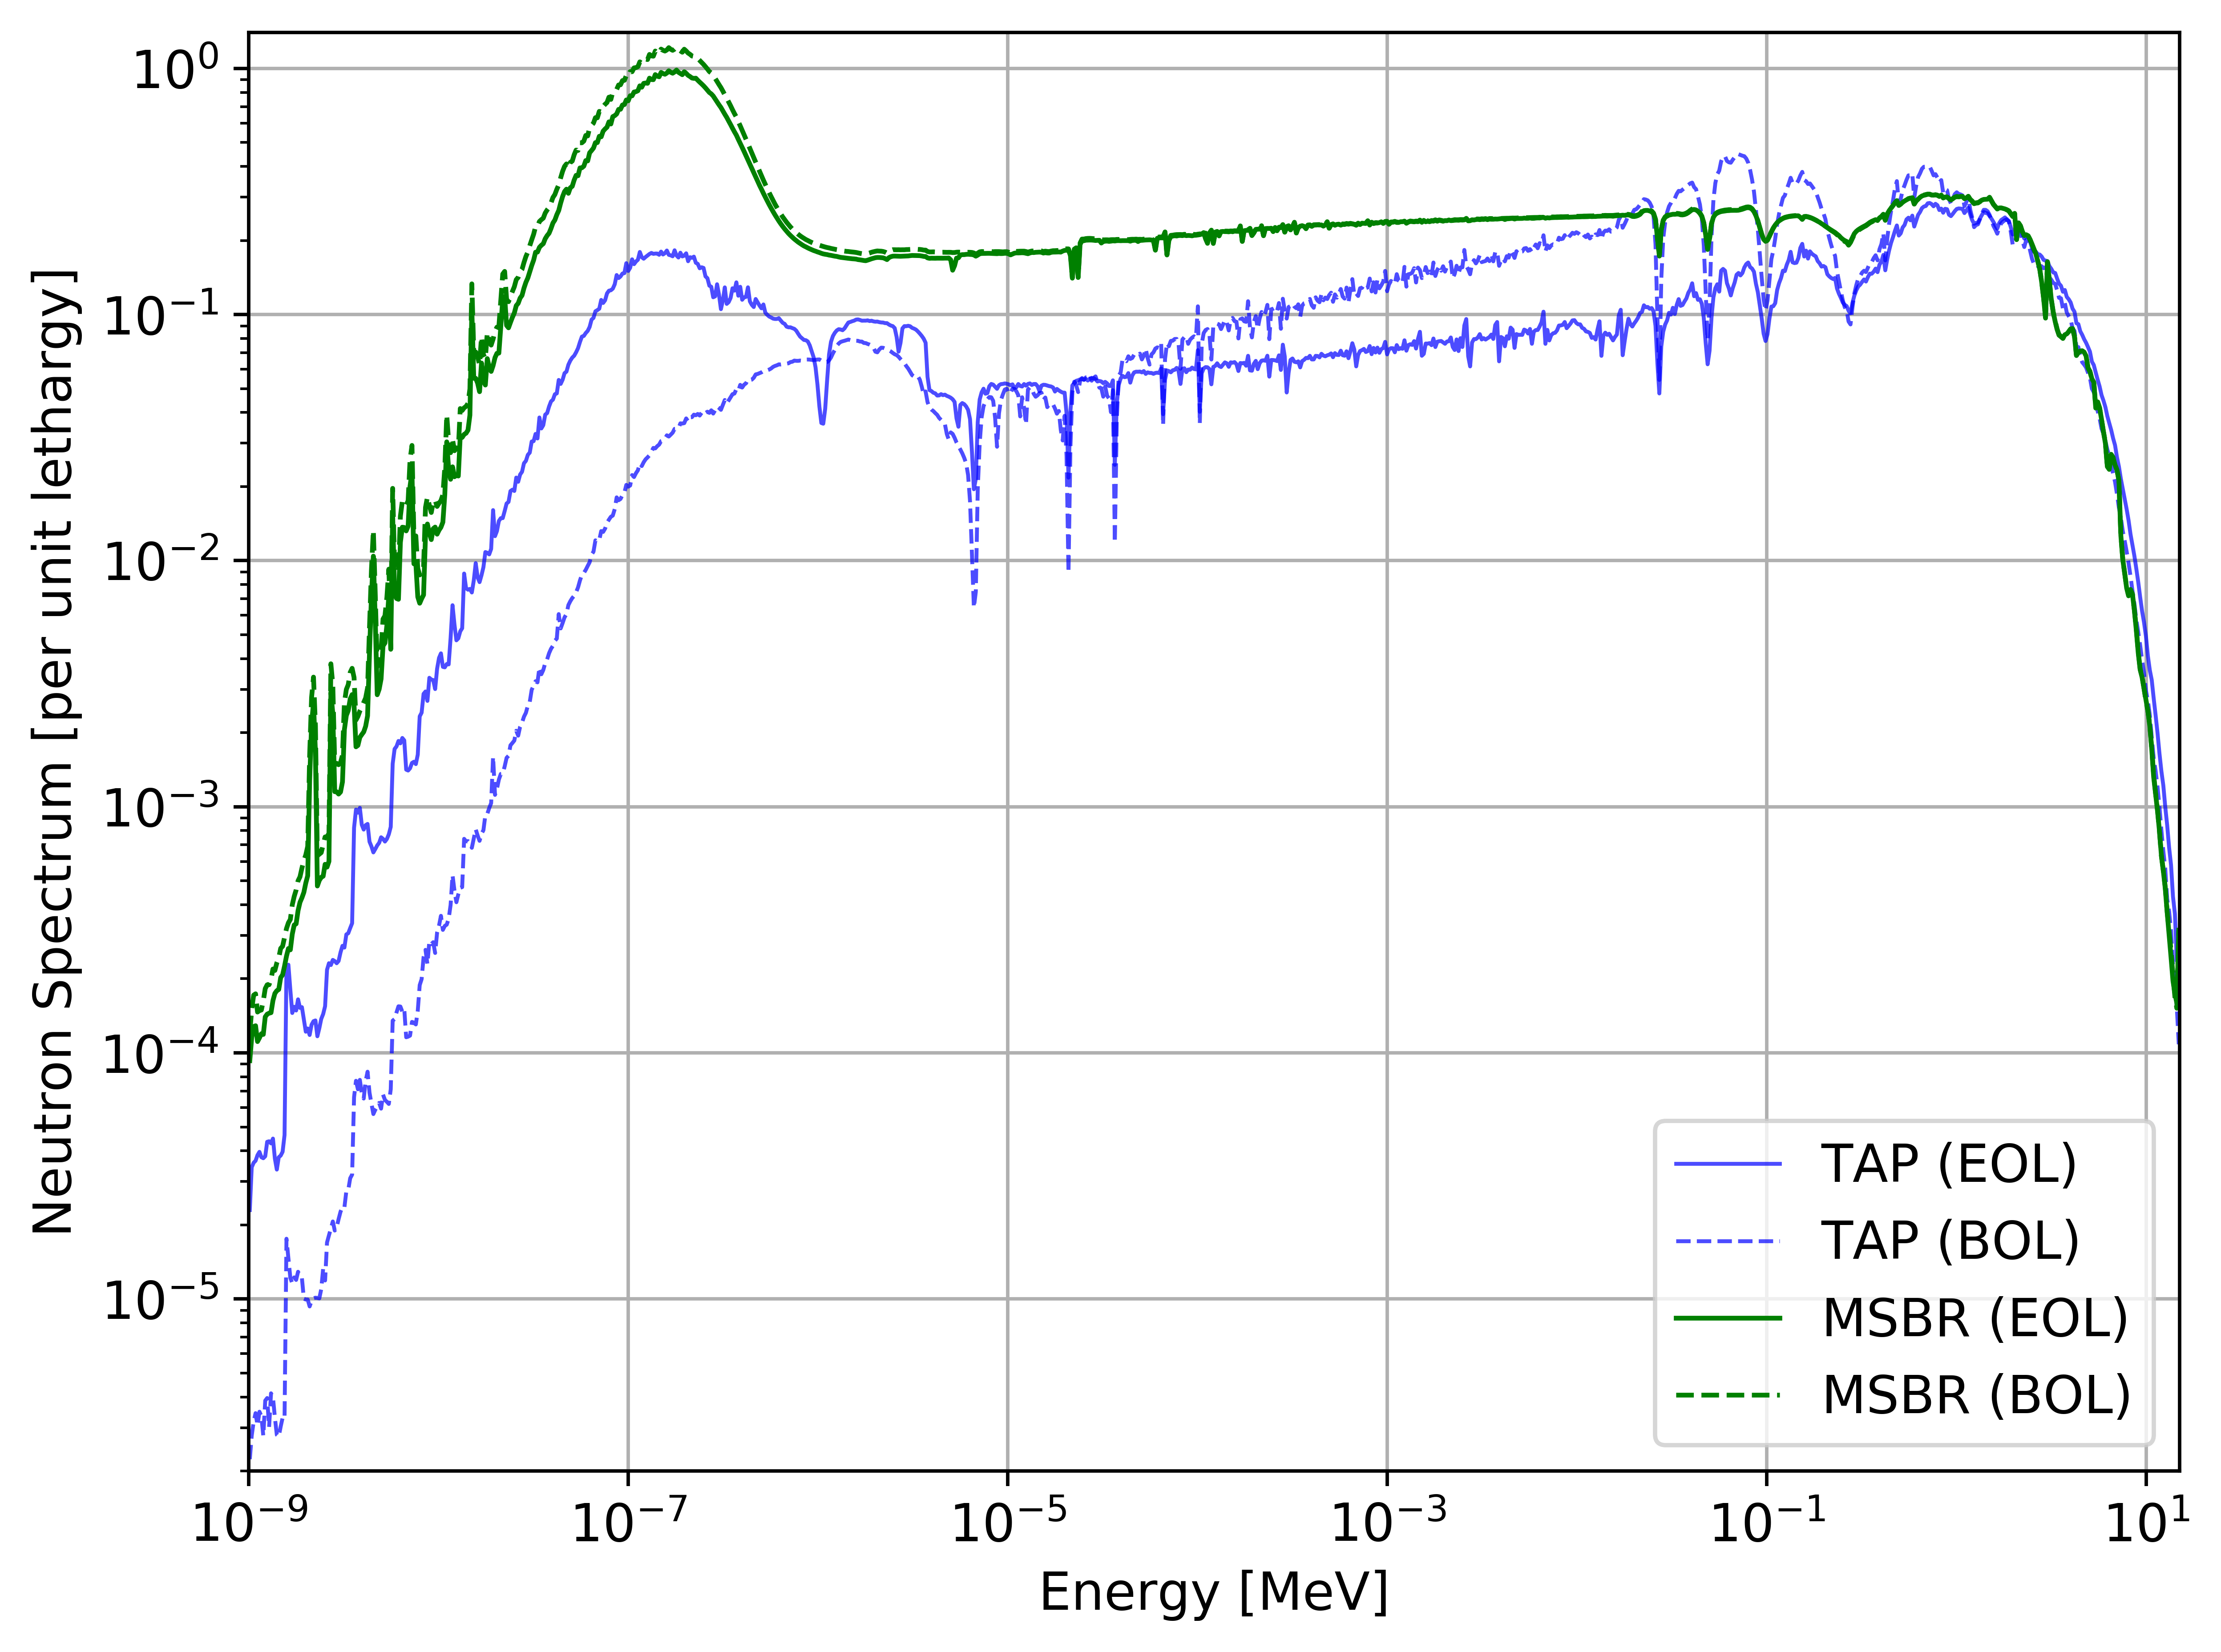
\includegraphics[width=0.73\textwidth]{../dissertation/figures/ch6/msbr_vs_tap_spectrum.png}}
		\vspace{-3mm}
		\caption{The neutron flux energy spectrum normalized by unit lethargy 
		for 
			MSBR and TAP at BOL and EOL. }
	\end{figure}
\end{textblock*}
\end{frame}